\chapter{MAGNETOSTATICS}
We have been discussing electrostatics, which deals with electric field created by static charges. Now it's time to look into a different phenomenon, the production and properties of magnetic field, whose source is steady current, i.e., charges in motion. An essential difference between the electrostatics and magnetostatics is that electric charges can be isolated, i.e., there exist positive and negative charges which can exist by themselves. Unlike this situation, magnetic charges (which are known as magnetic monopoles) cannot exist in isolation, every north magnetic pole is always associated with a south pole, so that the net magnetic charge is always zero.\\
Sources of magnetic field are steady currents. In such a field a moving charge experiences a sidewise  force.  Recall that an electric field exerts a force on a charge, irrespective of whether the charge is  moving or static. Magnetic field, on the other hand, exerts a force only on charges that are moving.  Under the combined action of electric and magnetic fields, a charge experiences, what is known as Lorentz force.
\section{Lorent'z Force Law}
The magnetic force on a charge $Q$ moving with a velocity $V$ in a magnetic field $B$ is given by,
\begin{equation}\label{Lorent'z Force Law 1}
\vec{F}_{mag}=Q(\vec{V}\times \vec{B})
\end{equation}
An electric field exerts a force on a charge, irrespective of whether the charge is
moving or static. Magnetic field, on the other hand, exerts a force only on charges that are moving. In the presence at both electric and magnetic field, a charge experiences, what is known as Lorentz force,
The net force on $Q$ would be,
\begin{equation}\label{Lorent'z Force Law 2}
\vec{F}=Q[\vec{E}+\vec{V}\times \vec{B}]
\end{equation}
\subsection{Force on a Conductor in a Magnetic Field}
Lorentz force law deals with a point charge moving in a magnetic field. Now we are going to find the expression for  force on a conductor in a magnetic field having line charge density $\lambda$.\\
Consider the figure and a point p on it . Suppose we are measuring the flow of charges in a time intervel $\Delta t$ through the point p. Let the velocity of electrons be $\vec{V}$. Therefore the charge flowing through the point in $\Delta t$ time is $\lambda V \Delta t$. Since $\lambda$ is the line charge density. \\
\begin{minipage}{.65\textwidth}
	\begin{align*}
	\text{Current } I&=\frac{Q}{t}\\
	I&=\frac{\lambda \vec{V} \Delta t}{\Delta t}=\lambda \vec{V}
	\intertext{The magnetic force on a line segment of length $d l$ and charge $dq$ is given by Lorentz force law}
	\vec{F}&=(\vec{V} \times \vec{B}) d q=(\vec{V} \times \vec{B}) \lambda d l \quad \quad dq=\lambda dl\\
	\text{Total}\quad \vec{F}&=\int(\vec{V} \times \vec{B}) \lambda d l\\
	&=\int(I \times \vec{B}) d l=\int I(\vec{dl}\times \vec{B} ) \quad \quad I=\lambda \vec{V}\\
	F_{mag}&=I\int(\vec{dl}\times \vec{B})
	\end{align*}
\end{minipage}
\begin{minipage}{.40\textwidth}
	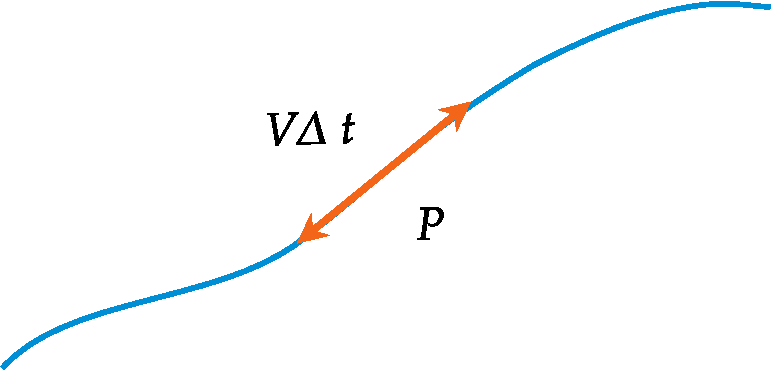
\includegraphics[height=3cm,width=5cm]{07-crop}
\end{minipage}
\subsection{Direction of Force: Fleming's Left Hand Rule (Motor Rule):}
\begin{minipage}{0.60\textwidth}
When a current carrying conductor is placed in an external magnetic field, the conductor experiences a force. The direction of the force is given be Fleming's left hand rule.\\ Stretch thumb, index finger, middle finger in 3 mutually perpendicular direction. If middle finger points in the direction of current and index finger in the direction of field. Then the direction of force is given by thumb.
\end{minipage}\hfil
	\begin{minipage}{0.25\textwidth}
	\begin{figure}[H]
		\centering
		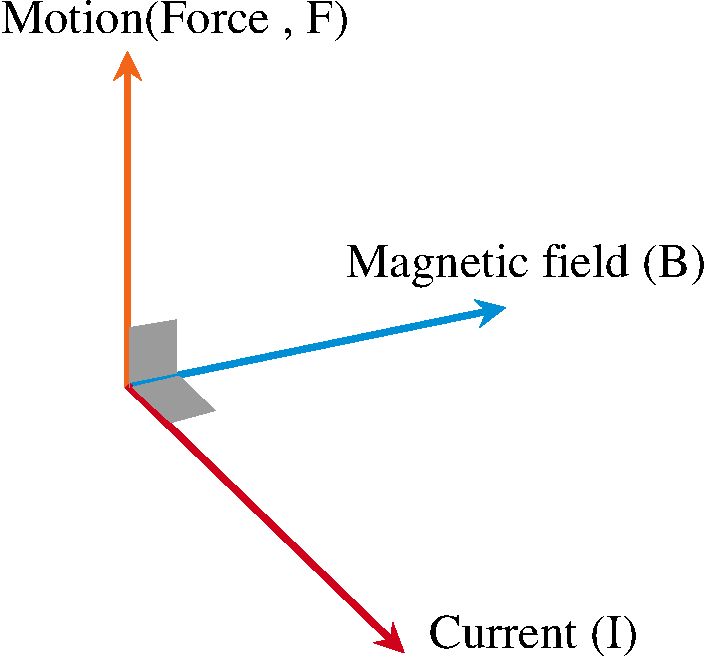
\includegraphics[height=3cm,width=3cm]{Flemings left hand rule}
		\caption{Flemings left hand rule}
		\label{Flemings left hand rule}
	\end{figure}
\end{minipage}
\subsection{Force on Surface With Surface Current Density K in a Magnetic Field}
If $d I$ is the small current through a ribbon on the surface and $d l_{\perp}$ is the perpendicular length then \\
\begin{minipage}{.40\textwidth}
	\begin{align*}
	\vec{K} \equiv \frac{d I}{d l_{\perp}}
	\end{align*}
\end{minipage}
\begin{minipage}{.30\textwidth}
	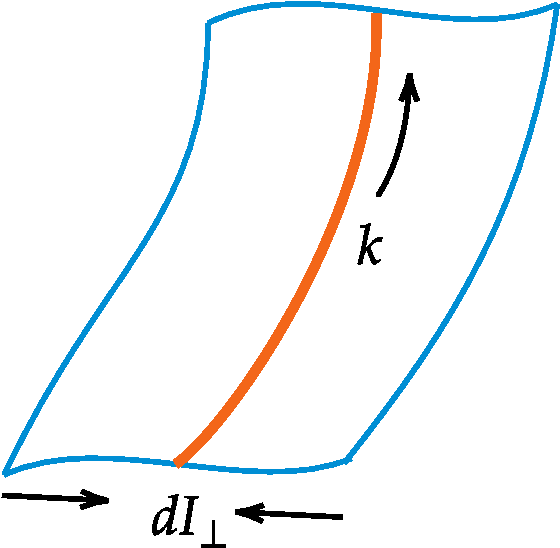
\includegraphics[width=0.6\textwidth]{08-crop}
\end{minipage}
\begin{align*}
\text{Which is the }&\text{current per unit width perpendicular to flow}\\
\text{But} \quad \vec{K}&=\sigma V\\
\text{Where} \quad \sigma&= \text{surface charge density}\\
\text{so magnetic }&\text{force on surface current is}\\
\vec{F}_{m a g}&=\int(\vec{V} \times \vec{B}) \sigma d a=\int(\vec{K} \times \vec{B}) d a
\end{align*}
\subsection{Force on a Volume With volume Current Density J in a magnetic field}
Consider a tube of infinitesmal cross section $da_\perp$ running parallel to the flow . If the current in this tube is $dI$ the volume current density is,\\
\begin{minipage}{0.6\textwidth}
\begin{align*}
\vec{J} &\equiv \frac{d I}{d a_{\perp}}\\
\text{$J$ is the current }&\text{per unit area - perpendicular to flow}\\
\vec{J}&=\rho \vec{V}\\
\rho&= \text{volume charge density}\\
\text{The magnetic force  on}&\text{ a volume current,}\\
F_{mag}&=\int(\vec{V} \times \vec{B}) \rho d \tau=\int(\vec{J} \times \vec{B}) d \tau
\end{align*}
\end{minipage}
\begin{minipage}{0.5\textwidth}
\begin{figure}[H]
	\centering
	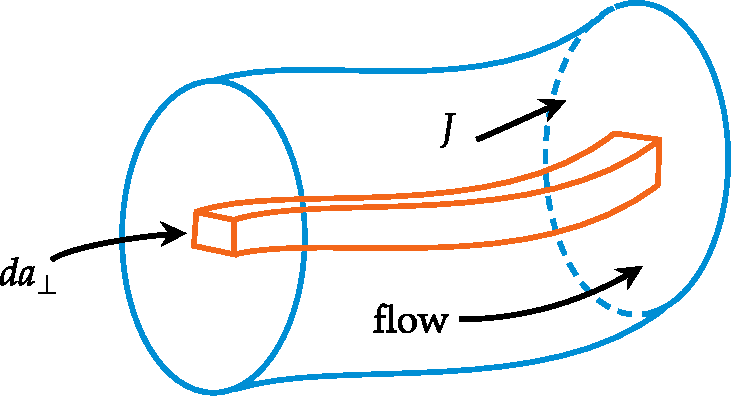
\includegraphics[height=3cm,width=5cm]{diagram-20220222(7)-crop-20220222162321}
	\caption{}
	\label{}
\end{figure}	
\end{minipage}
\subsection{Equation of Continuity}
Current is a scalar quantity which is the amount of charge that
crosses the boundary of a surface of a volume per unit time, the surface being oriented normal to the
direction of flow. In the steady state there is no accumulation of charge inside a volume through whose
surface the charges flow in. This results in the “equation of continuity” .
\begin{align*}
\vec{J}&=\frac{d I}{d a_{\perp}}\\
\text{so }&\text{current crossing a surface.}\\
I&=\int \vec{J} d a_{\perp}=\int \vec{J} \cdot d a\\
\text{current }&\text{through a closed surface $S$}\\
I&=\oint \vec{J} \cdot d a=\int_{V}({\nabla} \cdot {\vec{J}}) d \tau
\intertext{Because charge is conserved, whatever flows out through the surface must come at the expense of that remaining inside.}
\int_{V} \nabla \cdot \vec{J} d \tau&=\frac{-d}{d t} \int_{V} \rho d \tau=-\int \frac{\partial  \rho}{\partial  t} d \tau\\
\nabla\cdot \vec{J}&=-\frac{\partial  \rho}{\partial  t}\\
\nabla\cdot \vec{J}+\frac{\partial  \rho}{\partial  t}&=0\Rightarrow \text{  Continuity equation}
\intertext{The principle is a statement of conservation of electric charge.}
\end{align*}
\hspace{5.10cm}\framebox{
	
	\parbox[t][1.5cm]{4cm}{
		
		\addvspace{0.2cm} \centering 
		\textbf{Equation of continuity}\\ \vspace{0.2cm}
		$\nabla\cdot J+\frac{\partial  \rho}{\partial  t}=0$} 
}
\begin{note}
	When a steady current flows in a wire, its magnitude $I$ must be same all along the line. Otherwise the charge would be piling up some where, it wouldn't be a steady current. That is $\frac{d \rho }{d t}=0$ for steady current then.
	$$\nabla \cdot \vec{J}=0$$
	Steady current produces magnetic field that are constant in time.
\end{note}
\section{Biot Savart law}
 \begin{wrapfigure}{r}{0.25\textwidth}
	\begin{center}
		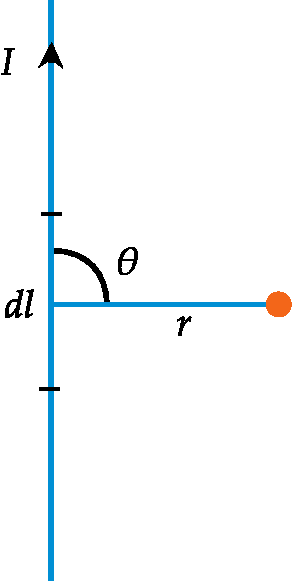
\includegraphics[width=0.15\textwidth]{diagram-20210417(4)-crop}
	\end{center}
	\caption{Biot Savart law}
\end{wrapfigure}
Magnetic field due to a steady current ${(\frac{d\rho}{dt}=0)}$\ is given by Biot Savart law.
The magnetic field at any point $P$ due to the current can be calculated by adding up the magnetic field contributions, $d \vec{{B}}$, from small segments of the wire $d \vec{l}$.
	\\Suppose we have a current carrying conductor having current '$I$' flowing through it. If $dl$ is the small length element on it. Then the magnetic field $\vec{B}$ at any point at a distance $r$ from $dl$ is given by,
	\begin{equation}\label{key}
	\vec{dB}={\frac{\mu_0}{4\pi}\frac{Idl\times{\hat{r}}}{r^2}}=\frac{\mu_0}{4\pi}\frac{Idl\sin\theta}{r^2}\qquad \vert{\hat{r}\vert}=1
	\end{equation}
	Where $\theta$ \ is the angle between $I$ and the distance $r$ . So the direction of magnetic field is $\perp^r$\ to both $dl$\ and $dr$. \\Then the magnetic field due to whole wire is ,
		\begin{equation}\label{key}
		B=\frac{\mu_0}{4\pi}\int\frac{Idl\times\hat{r}}{r^3}
		\end{equation}
 Where $\mu_0$ is the permeability of free space, $ \mu_0=4\pi\times10^{-7}\frac{N}{A^2}$\\
Unit of\ $B =N/A.m $\ or Tesla $T$
	\begin{alignat*}{2}
	&\textbf{For surface current:}\quad  &&B=\frac{\mu_0}{4\pi}\int\frac{k\times\hat{r}}{r^2}da\\ 
	&\textbf{For volume current J:}\quad  &&B=\frac{\mu_0}{4\pi}\int\frac{J\times\hat{r}}{r^2}d\tau \quad \text{or}\quad B=\frac{\mu_0}{4\pi}\int\frac{J\times\vec{r}}{r^3}d\tau\\
	\end{alignat*}
\begin{note}
	\begin{enumerate}
		\item Biot Savart law cannot be applied to a moving point charge.  Because a moving point charge can't be considered as steady current.
		
		\item The direction of magnetic field around a current carrying conductor is given by Right hand thumb rule,which states that when you hold the conductor in your right hand pointing thumb in the direction of current then your fingeres curl around the direction of magnetic field.\\
		
		
		\begin{figure}[H]
			\begin{minipage}{0.45\textwidth}
				\centering
				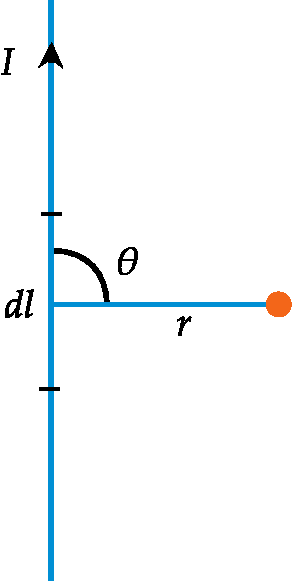
\includegraphics[height=4cm,width=2.2cm]{diagram-20210417(4)-crop}
			\end{minipage}
			\begin{minipage}{0.45\textwidth}
				\centering
				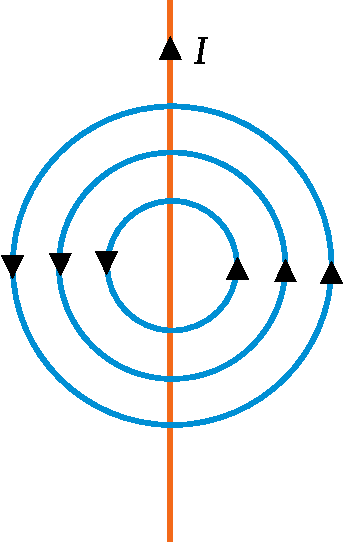
\includegraphics[height=4cm,width=2.7cm]{diagram-20210417(5)-crop}
			\end{minipage}
			\caption{}
			\label{parellel}
		\end{figure}	 
	\end{enumerate}
	
\end{note}

\subsection{Applications of Biot-Savart law}
\subsubsection{Magnetic field due to a long straight wire.}
Let us consider a long straight wire carrying a steady current I. We need to find the magnetic field $B$ a distance S from the wire.
\begin{figure}[H]
\begin{minipage}{0.45\textwidth}
	\centering
	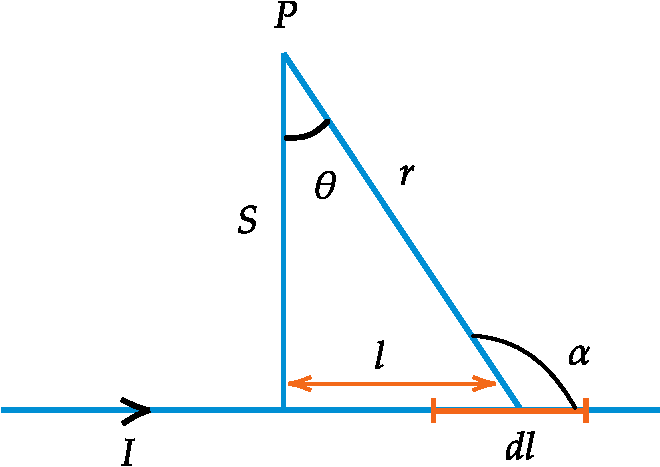
\includegraphics[height=4cm,width=5cm]{diagram-20210417(6)-crop}
\end{minipage}
\begin{minipage}{0.45\textwidth}
	\centering
	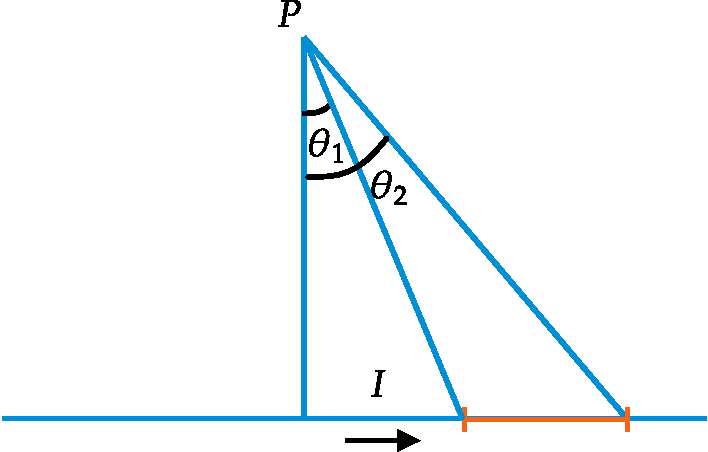
\includegraphics[height=4cm,width= 5cm]{diagram-20210417(7)-crop}
	\end{minipage}
\caption{Magnetic field due to line element.}
\label{Magnetic field due to line element}
\end{figure}
\begin{align*}
\text{Field due to a small }&\text{length element in figure \ref{Magnetic field due to line element}}\\
dB &=\frac{\mu_0}{4\pi}\frac{Idl\sin\alpha}{r^2}\qquad
 \Rightarrow\alpha=\theta+90\\
dl\sin \alpha &=dl\cos\theta\\
l&=S \tan\theta\\
\text{Integrating,}\quad dl &=\frac{S}{\cos^2\theta}d\theta\\
\text{And}\quad S&=r\cos\theta\\
\therefore\frac{1}{r^2}&=\frac{\cos^2\theta}{S^2}\\
\therefore dB=\frac{\mu_0}{4\pi}\frac{Idl\cos\theta}{r^2}&=\frac{\mu_0}{4\pi}\frac{ISd\theta}{\cos^2\theta}\times\frac{\cos^2\theta}{S^2}\times\cos\theta\\
&=\frac{\mu_0I}{4\pi S}cos\theta d \theta
\intertext{When we consider a wire segment  making an angle $\theta_1$,and $\theta_2$ with the point $P$ then $B$ is given by integrating between the limits  $\theta_1$,and $\theta_2$}
B&=\frac{\mu_0I}{4\pi S}\int\cos d \theta_2\\
B&=\frac{\mu_0I}{4\pi S}[\sin\theta_2-\sin\theta_1]
\end{align*}

\hspace{5.10cm}\framebox{
	
	\parbox[t][2.0cm]{7cm}{
		
		\addvspace{0.2cm} \centering
	\textbf{	Magnetic field due to a long straight wire.} \\ \vspace{0.4cm}
		$B=\frac{\mu_0I}{4\pi s}[\sin\theta_2-\sin\theta_1]$} 
}
\opencutright
\renewcommand\windowpagestuff{
	\centering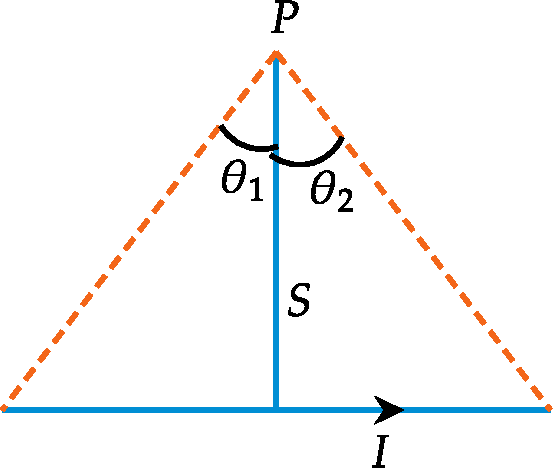
\includegraphics[height=3cm,width= 4cm]{12-crop}}
\begin{note}
	\vspace{0.5cm}
	\begin{cutout}{3}{\dimexpr\linewidth-7cm\relax}{0pt}{1}
		{\textbf{ For an infinite wire:}}
	\begin{align*}
	\theta_{1}&=\frac{-\pi}{2}\quad ; \quad
	\theta_{2}=\frac{\pi}{2}\\\\
	B&=\frac{\mu_{0} I}{4 \pi s}\left(\sin \frac{\pi}{2}-\sin \frac{-\pi}{2}\right)\\
	&=\frac{\mu_{0} I}{4 \pi s}\times2
  \\&=\frac{\mu_{0} I}{2 \pi s}
	\end{align*}
	Thus for an infinitely long wire the magnetic field, 
	\begin{equation*}
	B=\frac{\mu_{0} I}{2 \pi s}
	\end{equation*}
	\end{cutout}
\end{note}
\subsubsection{Magnetic field due to a circular loop.}
 Let us consider a circular loop of radius $ R  $\ which carries a steady current I, the magnetic field a distance $ z $ above the center

\begin{minipage}{0.55\textwidth}
\begin{align*}
	\intertext{Magnetic field at $P$ due to $dl$ is given by,}
	d \vec{B}&=\frac{\mu_{0}I}{4 \pi} \frac{ d \vec{l} \times \vec{a}}{a^{3}}\hspace{2cm} \begin{array}{cc}
	dl\perp a\\
	\therefore\sin90=1
	\end{array}\\
	d \vec{B}&=\frac{\mu_{0}I}{4 \pi} \frac{ d {l} }{a^{2}}
	\end{align*}
\end{minipage}
\begin{minipage}{0.35\textwidth}
	\centering
	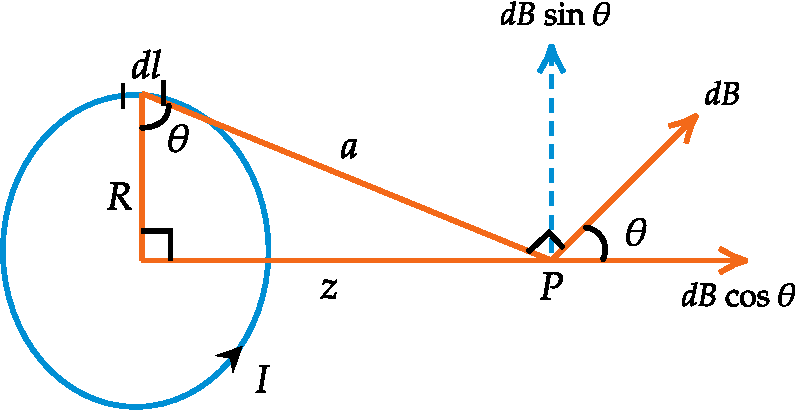
\includegraphics[height=3.2cm,width= 6cm]{diagram-20210420-crop}
\end{minipage}\\\\
$dB$ resolved in to two component $dB \cos \theta, dB \sin \theta $ due to symmetry the vertical components cancel and the horizontal components combine to give the total magnetic field $B$,
	

\begin{minipage}{0.60\textwidth}
	\begin{align*}
		B&=\int dB \cos \theta\\
	B&=\frac{\mu_0I}{4\pi} \int \frac{dl \cos \theta}{a^2}
	\intertext{$\cos \theta$ \ and \  $a^2$ are constants and $\int dl$ is simply the circumference $2\pi r$.}
	\therefore B&=\frac{\mu_0 I}{4\pi} \frac{\cos \theta}{a^2}\times 2\pi R\\
	\therefore B&=\frac{\mu_0 I}{4\pi}\frac{R^2\times2\pi}{(R^2+z^2)^\frac{3}{2}}\\  \therefore B&=\frac{\mu_0 I}{2} \frac{R^2}{(R^2+z^2)^\frac{3}{2}}
	\end{align*}
\end{minipage}
\begin{minipage}{0.40\textwidth}
		\vspace{3cm}
	\begin{align*}
	\text{but,}\quad
	\cos \theta &=\frac{R}{a}\\
	\cos \theta &=\frac{R}{(R^2+z^2)^\frac{1}{2}}\\
	a&={(R^2+z^2)^\frac{1}{2}}\\
	a^2&={(R^z+z^2)}
	\end{align*}
\end{minipage}
\begin{corollary}\hspace{0.5cm}
	\begin{enumerate}
		\item At the center of the circle
		\begin{align*}
		B&=\frac{\mu_0 I}{2}\frac{R^2}{(R^2+z^2)^\frac{3}{2}}\\
		\text{At center }\ z&=0\\
		B&=\frac{\mu_0 I}{2 R}
		\end{align*}
		\item When there are n no of turns,
		\begin{align*}
		B&=\frac{\mu_0 n I}{2 R} \ \ \ (\text{At center} ) 
		\end{align*}
	\end{enumerate}
\end{corollary}
\subsection{Some important results}
\begin{enumerate}
	\item Important Points
	When two circular coils of radius $r_{1}$ and $r_{2}$, having same material and same number of turns are connected in series, the current through each coil is same, the ratio of the magnetic field induction at their centre is given by
	$$
	\frac{B_{1}}{B_{2}}=\frac{r_{2}}{r_{1}}
	$$
	\item If two solenoids having turns $N_{1}$ and $N_{2}$ are connected in series, then current is same in both. Then
	$$
	\frac{B_{1}}{B_{2}}=\frac{N_{1}}{N_{2}}
	$$
	\item If a current $i$ flows through a circular path of radius $r$ which subtends an angle $\alpha$ (in radius) at the centre, as shown in figure, the magnetic field induction at the centre $O$ is given by $B=\frac{\mu_{0}i}{2r} \frac{\alpha }{2\pi}$.
		\begin{figure}[H]
		\begin{center}
			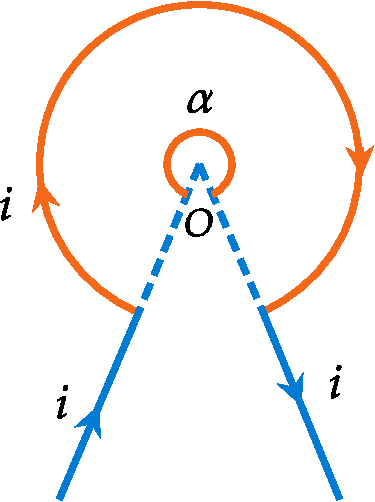
\includegraphics[width=0.15\textwidth]{field}
		\end{center}
	\end{figure}
\end{enumerate}
\begin{exercise}
	Find the magnetic field $B$ at the center of a squar loop of side $a$,if current I is flowing in the anticlockwise direction.which is the result when we consider a finite length.
\end{exercise}
\opencutright
\renewcommand\windowpagestuff{
	\centering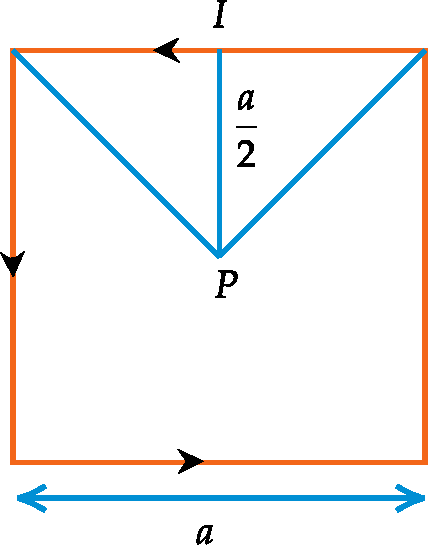
\includegraphics[width=2cm]{diagram-20210417(9)-crop}}
\begin{answer}
	\vspace{1cm}
	\begin{cutout}{3}{\dimexpr\linewidth-6cm\relax}{0pt}{6}
		\begin{align*}
		B\ \text{at}\  P\ &\text{due to one side,}\\
		B&=\frac{\mu_0I}{4\pi \frac{a}{2}}[\sin\theta_2-\sin\theta_1]\\
		\theta_1&=-45 \quad \theta_2=45\\\\
		B&=\frac{\mu_0I}{4\pi \frac{a}{2}}\times\frac{2}{\sqrt{2}}=\frac{\mu_0I}{\pi a}\times\frac{1}{\sqrt{2}}\\
		\text{So total }&\text{field at P,}\\
		B&= 4\times\frac{\mu_0I}{\pi a} \times \frac{1}{\sqrt{2}}=\frac{2\sqrt{2}\mu_0I}{\pi a}
		\end{align*}
	\end{cutout}
\end{answer}


\begin{exercise}
	Find the field at the center of a regular $n$ sided polygon carrying a steady current $I$. $R$ be the distance from center to any side.
\end{exercise}
\begin{answer}
	 for a $n$ sided polygon vertex of each side make an angle $\frac{\pi}{n}$ with center $P$ .\\
	 \begin{figure}[H]
	 	\centering
	 	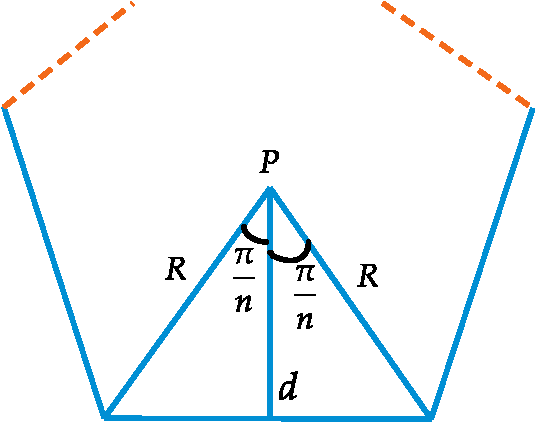
\includegraphics[height=3cm, width=3.5cm]{diagram-20210420(1)-crop}
	 \end{figure}
 
	\begin{minipage}{0.60\textwidth}\hfill
		\begin{align*}
		\therefore B&=n\times\frac{\mu_0 I}{4 \pi d}(\sin\frac{\pi}{n}-\sin\frac{-\pi}{n})\\
		&=n\times\frac{\mu_0 I}{4 \pi R \cos\frac{\pi}{n}}\times2 \sin\frac{\pi}{n}\\
		&=n\times\frac{\mu_0 I}{2 \pi R}\tan \frac{\pi}{n}\\
		&=\frac{\mu_0 I}{2 \pi R}\tan \frac{\pi}{n}
		\end{align*}
	\end{minipage}
	\begin{minipage}{0.40\textwidth}
		\begin{align*}
		\sin(-\theta)=-\sin \theta\\
		\cos\frac{\pi}{n}=\frac{d}{R}\\
		\therefore d=R\cos\frac{\pi}{n}
		\end{align*}
	\end{minipage}

	\begin{corollary}
		\begin{align*}
			\intertext{When $n =\infty$\  Polygon become circle.}
		\therefore \text{when}\	n\rightarrow\infty, \quad\tan\frac{\pi}{n}&=\frac{\pi}{n}\\
		\therefore B&=\frac{\mu_0 I}{2 \pi R}\frac{\pi}{n}\\&=\frac{\mu_0I}{2R} (\text{When , n=1})
		\end{align*}
	\end{corollary}
\end{answer}
\begin{exercise}
Find the magnetic field at point $P$ for each of the steady current configuration.\\
	(\textbf{a}) 
	\begin{minipage}{0.25\textwidth}\hfill
		\centering
		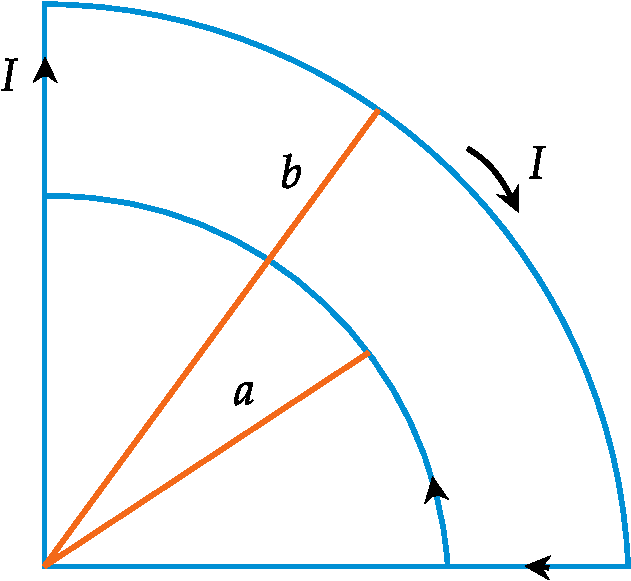
\includegraphics[width=0.75\textwidth]{diagram-20210420(2)-crop}
	\end{minipage} \hspace{2cm}
	(\textbf{b})
		\begin{minipage}{0.25\textwidth}\hfill
				\centering
			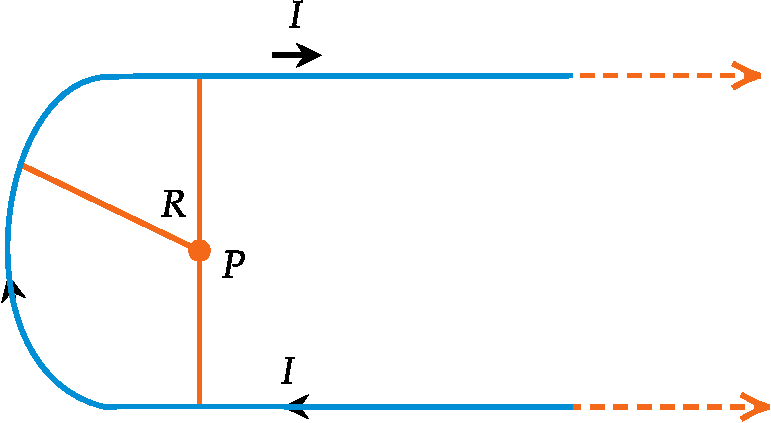
\includegraphics[width=1\textwidth]{diagram-20210421-crop}
		\end{minipage}
\end{exercise}
\begin{answer}
	\vspace{0.2cm}
	(\textbf{a})\\
	Magnetic field due to the segment at the end points of the annular region is zero. Because the magnetic field at  a point along the direction of a line segment is zero. Now we have to consider the two circular part.\\
  Field at $P$ due to part with radius $a$,
 \begin{align*}
 B&=\frac{1}{4}\times \frac{\mu_0 I}{2a}\quad \text{Out to plane of the paper}\\
 \text{field at }&\text{$p$ due to region $b$}\\
 B&=\frac{1}{4}\times \frac{\mu_0 I}{2b}\quad \text{In to the plane of the paper.}\\
 \therefore \quad\text{Total } &B\text{ at}\quad P =\frac{\mu_0 I}{4\times2}(\frac{1}{a}-\frac{1}{b})
 \end{align*}
	(\textbf{b})\\
	\begin{center}
		\begin{minipage}{0.45\textwidth}\hfill
			\centering
			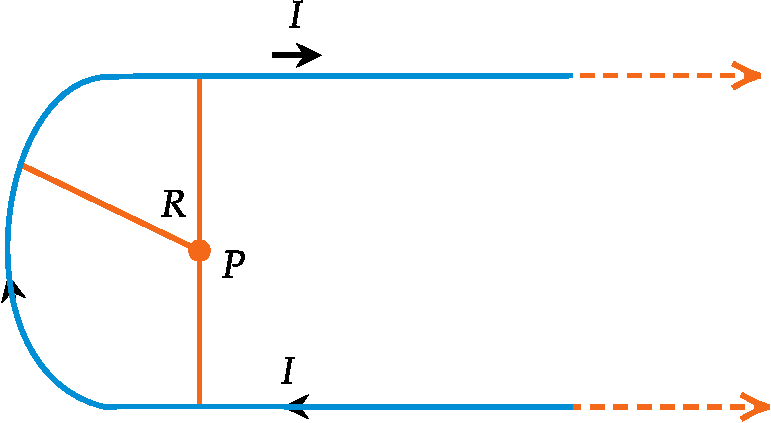
\includegraphics[height=2.5cm, width=4.5cm]{diagram-20210421-crop}
		\end{minipage}
		\begin{minipage}{0.45\textwidth}
			\centering
			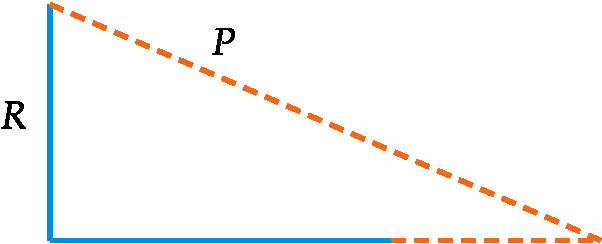
\includegraphics[height=3cm, width=4.5cm]{diagram-20210420(5)-crop}
		\end{minipage}
	\end{center}
	\begin{align*}
	\text{We can divide }&\text{the segment in to two part field at $P$ due to circular part is}\\
 B&=\frac{1}{2}\times \frac{\mu_0 I}{2R}=\frac{\mu_0 I}{4 R} \\
 \text{Field due to}&\text{ lower segment,}\\
B&=\frac{\mu_0 I}{4 \pi R}(\sin \theta_2-\sin \theta_1)  \qquad\begin{array}{l}
\text{Here,}\\\theta_1=0 \\
\theta_2=\frac{\pi}{2} 
\end{array}\\
\therefore B&=\frac{\mu_0 I}{4 \pi R}\\
\text{Field due }&\text{to the upper segment also equal to,}\\
B&=\frac{\mu_0}{4 \pi R}\\
\text{Field due to all the three }&\text{segment are directed in to the plane of thepaper. So}\\
B&=\frac{\mu_0 I}{4 R}+\frac{\mu_0 I}{4 \pi R}+\frac{\mu_0 I}{4 \pi R}\\
&=\frac{\mu_0 I}{4\pi R}(\pi+2)
\end{align*}
\end{answer}
\section{ Force Between Two Parallel Current Carrying Conductors}
\begin{enumerate}
	\item  The two long parallel conductors carrying currents in the same directions attract each other.And conductors carrying currents in the opposite direction repel each other.
	\item  The force acting per unit length of each conductor will be $F=\frac{\mu_{0}}{4 \pi} \frac{2 I_{1} I_{2}}{r}$
	\item  The force of attraction or repulsion acting on each conductor of length $l$ due to current in two parallel conductors is
	$$
	F=\frac{\mu_{0}}{4 \pi} \frac{2 I_{1} I_{2}}{r} l
	$$
	\item The force acting on two parallel current carrying conductors are equal in magnitude and opposite in direction.
	\item If two linear current carrying conductors of unequal length are held parallel to each other,then the force on a long conductor is due to magnetic field interaction due to currents of short and long conductor. If $l, L=$ length of short and long conductor respectively. $I_{1} \mathrm{I}_{2}=$  current through short and long conductors respectively and r is the seperation between these two parallel conductors ,\\
	for a long conductor$$B=\frac{\mu_{0}}{4\pi}\frac{2I_1I_2}{r}l$$
	\item  when two currents approach a point or they go away from that point, then they experience an altactive force.
	\item when one current out of the two, approaches a point and another one goes away from that point, then they experience a force of repulsion.
	\item If $q_{1}$ and $q_{2}$ are of the same nature and they move in the same direction, then the force acting between them is attractive.
	\item If $q_{1}$ and $q_{2}$ are of the same nature and they move in the opposite directions then the force acting between them is repulsive.
\end{enumerate}
\begin{exercise}
	A square loop is placed near a infinte stright wire as shown in figure.The loop and wire carry a steady current $I_2$ and $I_1$ respectively.Then the net force acting on the square loop?
	\begin{figure}[H]
		\centering
		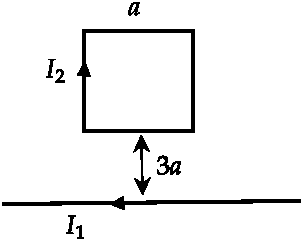
\includegraphics[height=3cm,width=5cm]{probs-crop}
	\end{figure}
\end{exercise}
\begin{answer}
	\begin{align*}
\text{	The force on two sides cancels.}\\
\text{	At the bottom,}B&=\frac{\mu_{0} I}{2\pi 3a} \implies F=\left[ \frac{\mu_{0} I_1}{6\pi a}\right] 	I_2a=\frac{\mu_{0} I_1I_2}{6\pi} \textbf{Down}\\
	\text{At the top, }B&=\frac{\mu_{0}I_1}{2\pi(3a+a)}\implies F=\frac{\mu_{0}I_1I_2a}{8\pi a}\implies F=\frac{\mu_{0}I_1I_2}{8\pi} \textbf{up}\\
\text{	Thus net force}&=\left( \frac{\mu_{0}I_1I_2}{6\pi}-\frac{\mu_{0}I_1I_2}{8\pi}\right) =\frac{\mu_{0}I_1I_2}{24\pi}\textbf{down}
	\end{align*}
\end{answer}
\section{Ampere's law}
 \begin{wrapfigure}{r}{0.35\textwidth}
	\begin{center}
		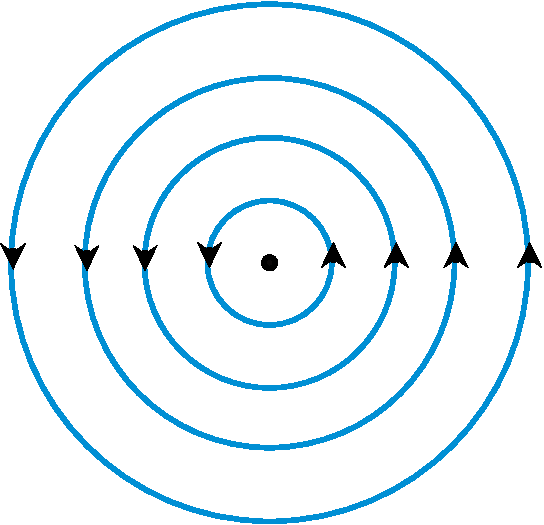
\includegraphics[width=0.25\textwidth]{diagram-20210421(1)-crop}
	\end{center}
	\caption{Amperes circuital law}
\end{wrapfigure}
Ampere's circuital law relates the net magnetic field along a closed loop to the electric current passing through the loop.
Consider the magnetic field produced by a infinite straight conductor having current coming out of the page. From that we can say that the curl of $B$ is not zero, but equal to $\mu_0J$

\begin{align*}
\therefore \nabla\times B&=\mu_0 \ J
\intertext{Which is called Ampere's law . It can be converted in to integral form by applying stoke's theorem.}
\int (\nabla\times B) \cdot d \tau&=\mu_0\int Jd\tau\\
\therefore \oint B \cdot dl&=\mu_0 I
\end{align*}
\begin{note}
	\textbf{1.} When the loop doesn't encloses the carrent carrying wire $d\phi=0$. Then Ampere's law can't be applied.\\
\begin{minipage}{0.25\textwidth}
	
\end{minipage}\hspace{10cm}	\begin{minipage}{0.25\textwidth}
		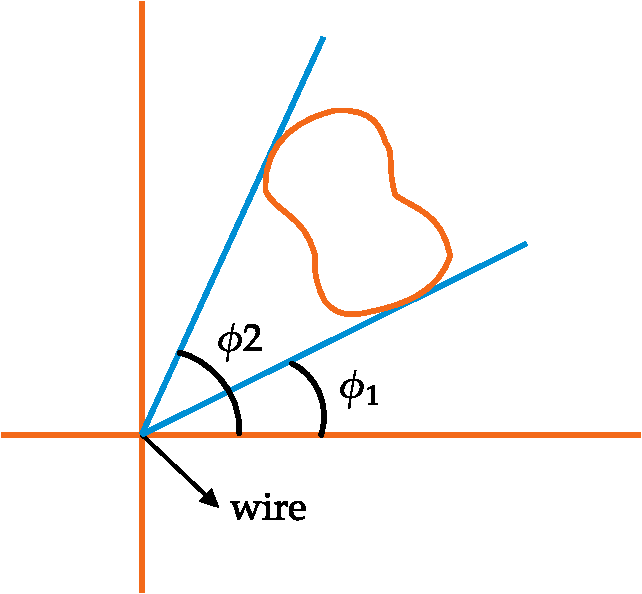
\includegraphics[height=4cm, width=4cm]{diagram-20210421(3)-crop}
	\end{minipage}\\\\
\textbf{2.} Suppose if we have a loop containing a no of current carrying wires then.\\\\
	\begin{minipage}{0.25\textwidth}
\begin{align*}
\oint B\cdot dl=\mu_0 I\quad\text{enclosed}\\
I_{enc}=I_1+I_2+I_3+I_4
\end{align*}
	\end{minipage}\hspace{2cm}
\hspace{4cm}	\begin{minipage}{0.25\textwidth}
		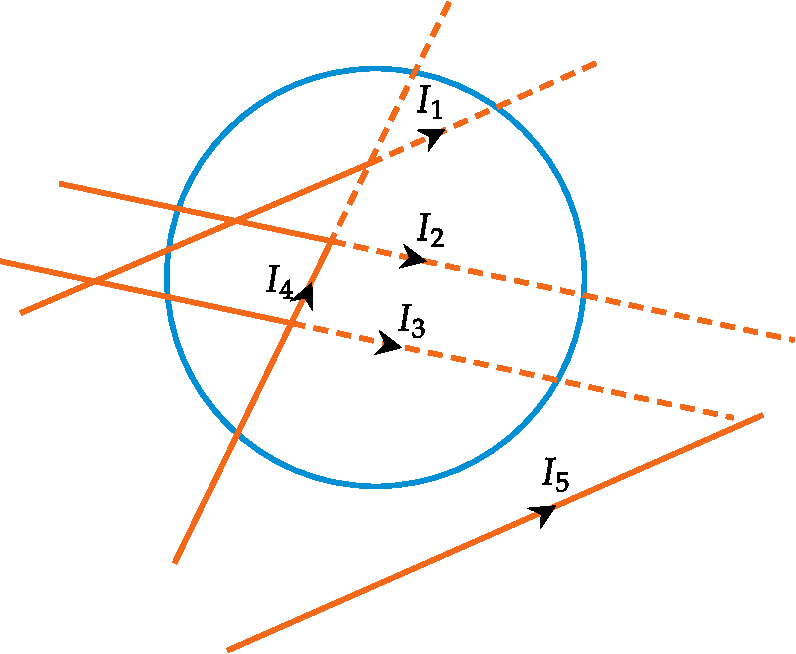
\includegraphics[height=3.5cm, width=4cm]{diagram-20210421(4)-crop}
	\end{minipage}\\
\textbf{3.} From Ampere's law and Biot Savart law we will obtain the divergence of $B$ is equal to zero.
$$\text{i.e.}\ \nabla \cdot B=0$$\\
i.e. if the magnetic field has started some where it will end some where.\\\\
\textbf{4.} Ampere's law is always true,But can mostly applied only to infinite current carying materials like 
Infinite straight lines,  Infinite planes, Infinite solenoids  ,Toroids
\end{note}
\subsection{Applications}
\subsubsection{Magnetic field of a long straight wire. }
To find the field at $P$ at a distance $r$ from the wire, consider an Amperial loop around the conductor having radius equal to $r$.\\
\begin{minipage}{0.65\textwidth}
\begin{align*}\\
\text{From Ampere's law }\\
\oint B\cdot dl&=\mu_0 I\\
\text{Since}\ B \ \text{and} \ dl \text{are parallel} , &B\text{can be pulled out of the integral so.}\\
B\oint dl&=\mu_0 I \hspace{2cm} \\ \oint dl&=2\pi r\\
B&=\frac{\mu_0 I}{2\pi r}
\end{align*}
\end{minipage}
\begin{minipage}{0.35\textwidth}
	\begin{figure}[H]
		\centering
		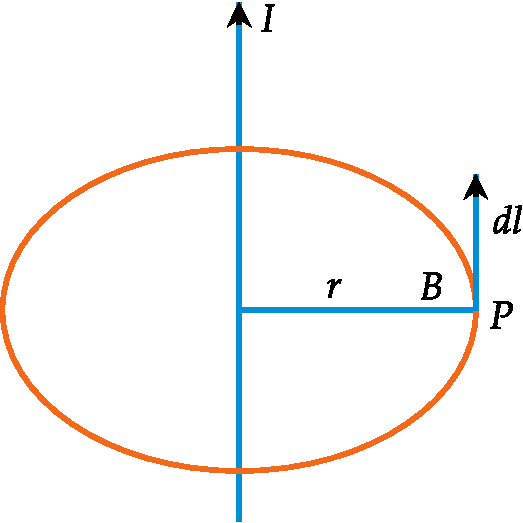
\includegraphics[height=4cm,width=4cm]{diagram-20210422(1)-crop}
		\caption{Long straight wire carrying current I}
		\label{Long straight wire}
	\end{figure}
\end{minipage}


Which is the same result that we got by using Biot-Savart law. But in this case Ampere's law is simpler.\\
\subsubsection{Magnetic field of a long Infinite sheet of current. }
\begin{wrapfigure}{r}{0.30\textwidth}
	\begin{center}
		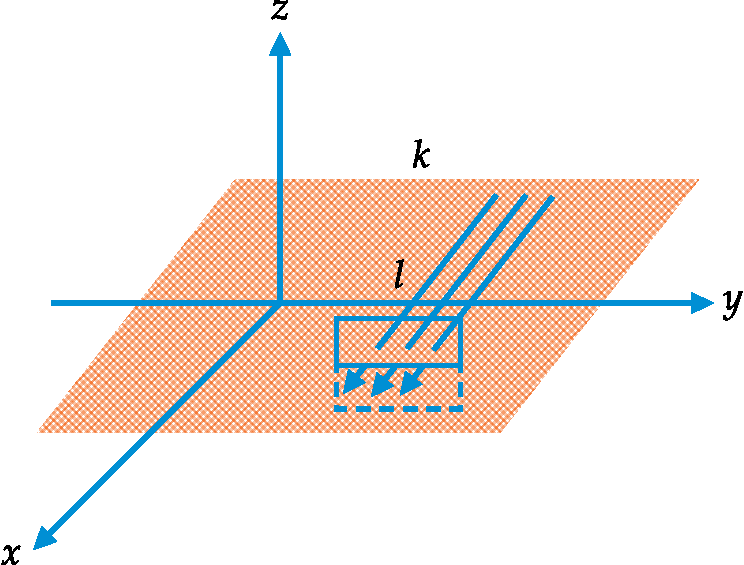
\includegraphics[height=4cm,width=6cm]{diagram-20210422(2)-crop}
	\end{center}
	\caption{Long Infinite sheet of current}
\end{wrapfigure}
Let us find the magnetic field of an infinite uniform surface current $k=k\hat{x}$ flowing over the $xy$ plane\\
By Biot-Savart law magnetic surface due to a surface current density $k$ is given by.
	\begin{align*}
	B&=\frac{\mu_0 I}{4\pi}\int\frac{k\times \hat{r}}{r^2}da\\
	k&=k\hat{x} 
	\end{align*}
When we consider the magnetic field at distance $r$ above and below the surface,$\hat{r}$\ is in $\hat{z}$ direction and $k$ along $\hat{x}$ direction and from Biot-Savart law $B$ is $\perp^r$ to both $\hat{x}$ and $\hat{z}$ direction. So it should be in $y$ direction.\\
Now consider a rectangular Amperian loop of length $l$ above and below the surface and parallel to $yz$ plane. Applying Ampere's law we find,
\begin{align*}
\oint B \cdot dl&=2Bl=\mu_0 I_{enc} \qquad\begin{array}{l}
\oint dl=2l \\
I{_{enc}=kl}
\end{array}\\
2Bl&=\mu_0kl\\
B&=\frac{\mu_0k}{2}
\end{align*}
By using right hand thumb rule, magnetic field above the surface is towards left ie$-y$ direction and $B$ below the surface is towards right ie $+y$ direction.\\\\
$f(x)= 
\begin{cases}
\frac{+\mu_0 k}{2}\hat{y}& \text{for }\ z<0\\\\
 \frac{-\mu_0 k}{2}\hat{y} & \text{for}\ z>0
\end{cases}$
\begin{note}\\
	$B$ is independent of distance from the plane.
\end{note}
\subsubsection{Magnetic field of a long  solenoid. }
A solenoid is essentially a long current loop with closely packed circular turns. The length of the solenoid  is very large compared to  the diameter of the turns. 
Let us find the magnetic field of a very long solenoid, consisting of $n$ closely wound turns per unit length on a cylinder of radius $R$ and carrying a steady current $I$.

\begin{minipage}{.45\textwidth}
\begin{figure}[H]
		\begin{center}
		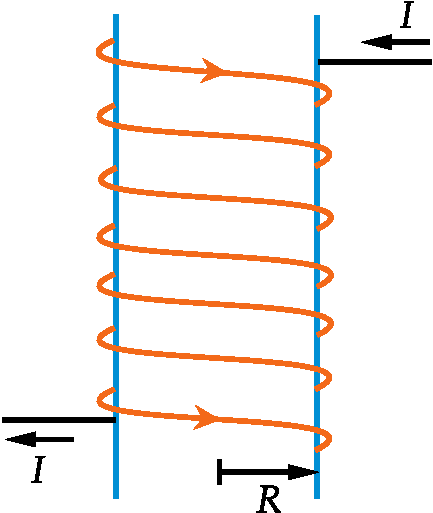
\includegraphics[width=0.4\textwidth]{diagram-20210422(3)-crop}
	\end{center}
\label{key}
\caption{Long solenoid}
	\end{figure}

\end{minipage}
\begin{minipage}{.45\textwidth}
	\begin{figure}[H]
		\begin{center}
			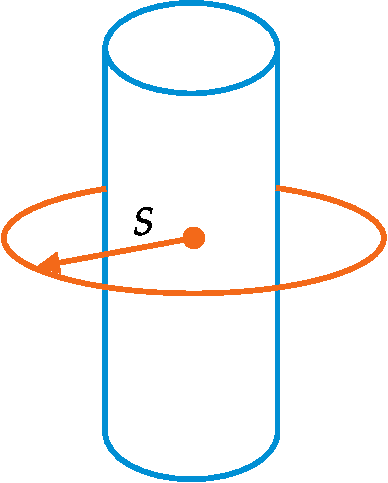
\includegraphics[width=0.4\textwidth]{diagram-20210422(4)-crop}
		\end{center}
	\label{key}
	\caption{Amperian loop}
	\end{figure}
\end{minipage}
\\\\Suppose the magnetic field \ $B$ is positive, then if we change the directions of current $B$ should be negative. Changing the direction of current is equivalent to turning the solenoid upside down. Then radial component won't change.\\
There will be no circumferential component for \ $B(\phi)$ \ also. Because when we consider an amperial loop around the solenoid, it has magnetic field parallel to the axis. It should be pointed upward inside the solenoid and downward outside. But now we can prove that $B$ outside the solenoid is also zero.\\
(We already know $B_\phi$ (circumferential component) is zero). For that now conside the loop $1$ of length $L$.\\
Applying Ampere's law to loop$1$\\
\begin{minipage}{0.65\textwidth}
	\begin{align*}
	\oint B\cdot dl&=B_a L-B_b L\\
	&=\mu_0 I_{enc} \hspace{2cm}I_{enc}=0\\
	&=0\\
	\therefore B_a&=B_b\\
	\therefore B\ &\text{is constant outside}
	\end{align*} 
\end{minipage}
\begin{minipage}{0.35\textwidth}
	\begin{figure}[H]
		\centering
		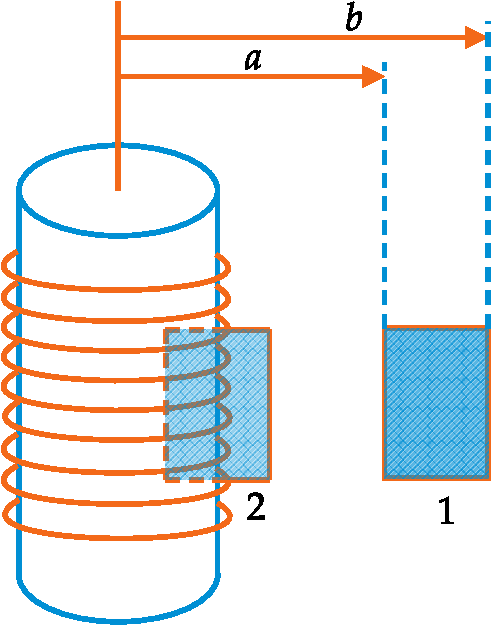
\includegraphics[height=4.5cm,width=4.5cm]{diagram-20210422(5)-crop}
		\caption{Amperian loop}
		\label{rc current discharge}
	\end{figure}	
\end{minipage}\\
\begin{align*}
\text{But a large distance }&\text{from solenoid $B$ must be zero. So it should be zero everywhere.}\\
\text{	For loop $2$ }&\text{half inside and half outside.}\\
\oint {B} \cdot d {l}&=B L=\mu_{0} I_{\mathrm{enc}}\\&=\mu_{0} n I L\\
B&= \begin{cases}
\mu_0 I \hat{z}& \text{inside}\\
0    & \text{outside}
\end{cases}
\end{align*}
\subsubsection{Magnetic field of Torroid. }
A torroid is a circular ring around which a long wire is wrapped. Suppose there are $N$ closely spaced wires find the magnetic field around the toroid at a distance $r$ from the center if $I$ is the current flowing through the torroid.
\begin{figure}[H]
\begin{minipage}{0.45\textwidth}
	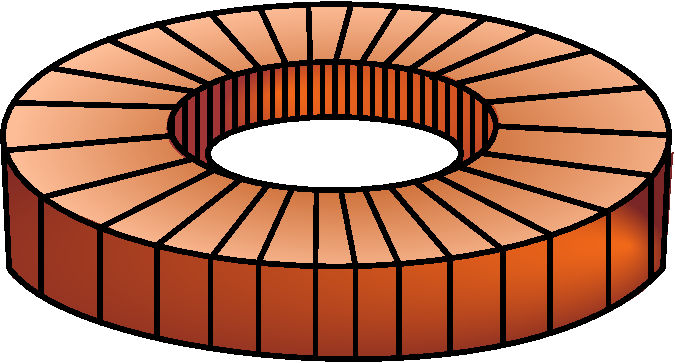
\includegraphics[height=2cm,width=5cm]{diagram-20210422(11)-crop}
\end{minipage}
\begin{minipage}{0.45\textwidth}
		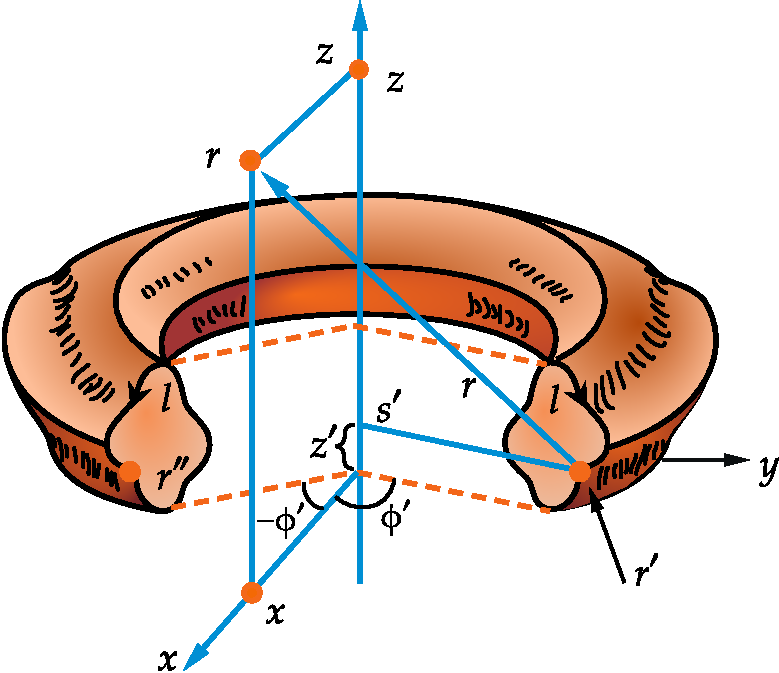
\includegraphics[height=4cm,width=5.5cm]{diagram-20210422(12)-crop}
\end{minipage}
\caption{Torroid}
\end{figure}
\begin{align*}
\intertext{Since the field is circumferential, determining its magnitude is ridiculously easy. Just apply Ampère's law to a circle of radius $s$ about the axis of the torroid:}
B 2 \pi s&=\mu_{0} I_{\text {enc }}\\
\text{And hence,}\ {B}(\mathbf{r})&=\left\{\begin{array}{cl}
\frac{\mu_{0} N I}{2 \pi s} \hat{\boldsymbol{\phi}}, & \text {For points inside the coil. } \\
0, & \text { For points outside the coil, }
\end{array}\right.
\text{Where $N$ is the total}&\text{ number of turns.}
\end{align*}
\begin{exercise}
	 A steady current $I$ flows down a long cylindrical wire of radius $a$ (Fig. 5.40). Find the magnetic field, both inside and outside the wire, if,
	\\(a) The current is uniformly distributed over the outside surface of the wire.
	\\(b) The current is distributed in such a way that $J$ is proportional to $s$, the distance from the axis.
\end{exercise}
\begin{answer}
	\begin{align*}
	\textbf{a)}\hspace{1cm}\quad\oint B \cdot d l&=B \times 2 \pi s=\mu_{0} I_{\text {encl }}\\
	B&=\left\{\begin{array}{ll}0 & \text { for } s<a \\ \frac{\mu _0 I}{2 \pi s} \phi & \text { for } s>a\end{array}\right.\\
	\textbf{b)}\hspace{2cm}\quad J&=k s\\
	I_{\text {Total }}&=\int_{0}^{a} J d a=\int_{0}^{a} k s 2 \pi s d s=\frac{2 \pi k a^{3}}{3}\\
	k&=\frac{3 I}{2 \pi a^{3}}\\
	I_{\text {encl }}&=\int_{0}^{S} k s(2 \pi s) d s\\
	&=\frac{2 \pi k s^{3}}{3}\\
	\text{Substituting }&\text{value of $k$.}\\
	I_{\text{encl}} &=\frac{I s^{3}}{a^{3}}\hspace{1.4cm}\text{ for } s<a\\
	I_{\text {encl }}&=I \hspace{1.8cm}\text{ for } s>a\\
	\therefore \quad B&=\left\{\begin{array}{l}\frac{\mu_{0} I s^{2}}{2 \pi a^{3}} \hat{\phi}\ \quad \text { for } s<a \\\\ \frac{\mu_{0} I}{2\pi s} \hat{\phi}\qquad \text { for } s>a\end{array}\right.
	\end{align*}
\end{answer}
\section{Magnetic Vector Potential}
In electrostatics, we had seen  a scalar function $\phi$ called the "potential"
whose negative gradient is equal to the electric field : 
\begin{equation*}
\vec{E}=-\nabla \phi
\end{equation*}
 The existence of such a scalar function is a consequence of the conservative nature of the electric force. It also followed that the electric field is irrotational, i.e.
 \begin{equation*}
\nabla \times \vec{E}=0
 \end{equation*}
For a magnetic field, Ampere's law gives a non-zero curl,
\begin{equation*}
\nabla\times \vec{B}=\mu_{0} \vec{J}
\end{equation*}

Since the curl of a gradient is always zero, we cannot express $\vec{B}$ as a gradient of a scalar function as it would then violate Ampere's law. However, we may introduce a vector function $\vec{A}(\vec{r})$ such that,

$$
\vec{B}=\nabla \times \vec{A}
$$
This would automatically satisfy $\nabla \cdot \vec{B}=0$ since divergence of a curl is zero.\ $ \vec{A} $\ is known as the vector potential.
\begin{center}
	\framebox{
		\parbox[t][0.75cm]{4cm}{
			
			\addvspace{0.2cm} \centering 
			
			$
			\vec{B}=\nabla \times \vec{A}
			$} }
\end{center}
\subsection{Biot-Savart's law for Vector potential.}
Biot-Savart's law for magnetic field due to a current element $\vec{d l}$\ is obtained as,
\begin{align*}
d \vec{B}&=\frac{\mu_{0} I}{4 \pi} \frac{\vec{d} l \times \hat{r}}{r^{2}}=-\frac{\mu_{0} I}{4 \pi} \vec{d} l \times \nabla\left(\frac{1}{r}\right)
\intertext{It can  be used to obtain an expression for the vector potential. Since the element $\overrightarrow{d l}$ does not depend on the position vector of the point at which the magnetic field is calculated, we can write}
d \vec{B}&=\frac{\mu_{0} I}{4 \pi} \nabla \times\left(\frac{\vec{d l}}{r}\right)\\
\text{The change in sign}&\text{ is because}\\
\nabla\left(\frac{d l}{r}\right)&=\nabla(1 / r) \times \vec{d l}\\
\text{Thus the contribution }&\text{to the vector potential from the element $\overrightarrow{d l}$ is, }\\
 d \vec{A}&=\frac{\mu_{0} I}{4 \pi r} \overrightarrow{d l}\\
 \text{The expression is to be integrated }&\text{over the path of the current to get the vector potential for the system}\\
 \vec{A}&=\frac{\mu_{0} I}{4 \pi} \int \frac{\vec{d} l}{r}
\end{align*}
\begin{center}
	\framebox{
		
		\parbox[t][1.0cm]{4cm}{
			
			\addvspace{0.2cm} \centering 
			$\vec{A}=\frac{\mu_{0} I}{4 \pi} \int \frac{\vec{d} l}{r}$} 
	}
\end{center}
\begin{exercise}
	A current distribution gives rise to the magnetic vector potential
	$$
	\vec{A}(x, y, z)=x^{2} y \hat{i}+y^{2} x \hat{j}-x y z \hat{k} 
	$$
	Find the corresponding magnetic field $\vec{B}$ at $(-1,2,5)$.
\end{exercise}
\begin{answer}
	\begin{align*}
	\vec{B}(x, y, z)&=\vec{\nabla} \times \vec{A}\\&=\left|\begin{array}{ccc}
	\hat{i} & \hat{j} & \hat{k} \\
	\frac{\partial}{\partial x} & \frac{\partial}{\partial y} & \frac{\partial}{\partial z} \\
	x^{2} y & y^{2} x & -x y z
	\end{array}\right|\\&=-x z \hat{i}+y z \hat{j}+\left(y^{2}-x^{2}\right) \hat{k}\\
	\vec{B}(-1,2,5)&=5 \hat{i}+10 \hat{j}+3 \hat{k} T
	\end{align*}
\end{answer}
\subsubsection{Vector potential due to a straight current carying wire.}
Let us consider a long straight wire $A B$ carrying a steady current $I$. We need to calculate the magnetic vector potential $\vec{\mathrm{A}}$ at any point $P .$ We choose cylindrical coordinates $(r, \theta, z)$ with z-axis along the wire and the foot $O$ of the perpendicular from $P$ on the wire as the origin. Let us consider an element $d \vec{l}=\hat{z} d z$ at a distance $z$ from $O$. Now by definition\\
\begin{minipage}{0.65\textwidth}
\begin{align*}
\vec{A}&=\frac{\mu_{0}}{4 \pi} \int \frac{I d \vec{l}}{R}=\hat{z} \frac{\mu_{0} I}{4 \pi} \int_{-l_{1}}^{+l_{2}} \frac{d z}{\sqrt{r^{2}+z^{2}}}\\&=\hat{z} \frac{\mu_{0} I}{4 \pi}\left[\ln \left(z+\sqrt{r^{2}+z^{2}}\right)\right]_{-l_{1}}^{+l_{2}}\\
&=\hat{z} \frac{\mu_{0} I}{4 \pi} l n\left[\frac{l_{2}+\sqrt{r^{2}+l_{2}^{2}}}{-l_{1}+\sqrt{r^{2}+l_{1}^{2}}}\right]
\end{align*}
\end{minipage}
\begin{minipage}{0.35\textwidth}
	\begin{figure}[H]
		\centering
		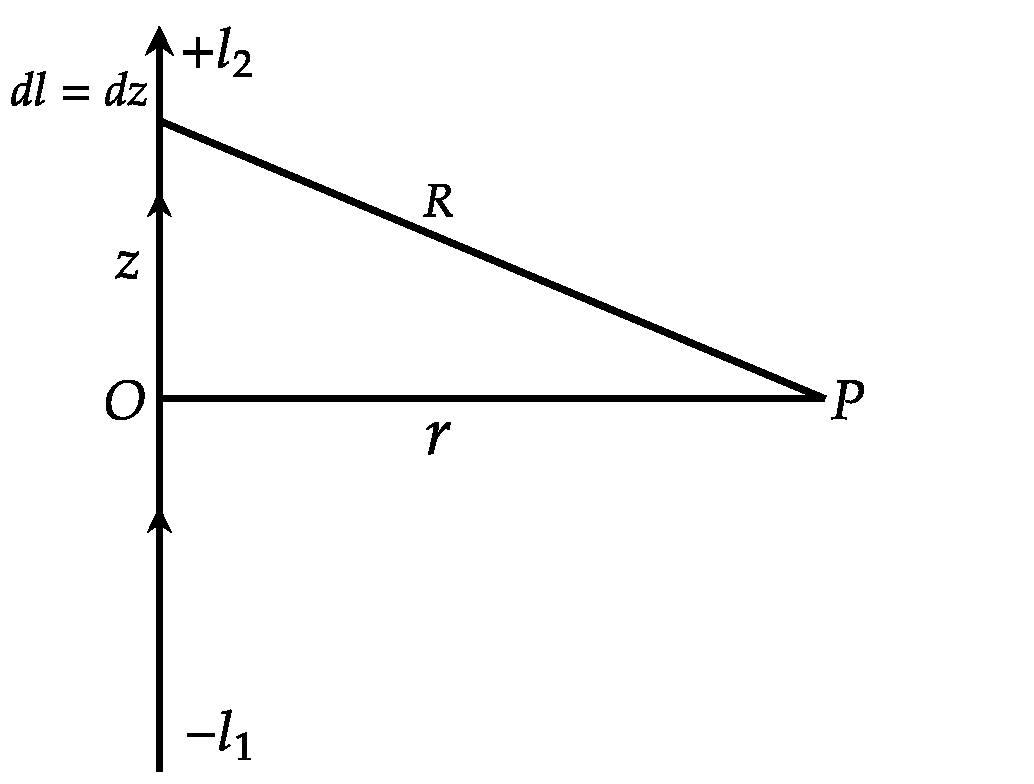
\includegraphics[height=5cm,width=6cm]{vector potential}
		\caption{Straight current carying wire.}
		\label{Straight current carying wire.}
	\end{figure}
\end{minipage}
\begin{align*}
\text{If the wire is of length $2 \mathrm{~L}$ and}&\text{  the point $\mathrm{P}$ is just above the centre of the wire then $l_{1}=l_{2}=L$ and we can write,}\\
\vec{A}&=\hat{z} \frac{\mu_{0} I}{4 \pi} \ln \left[\frac{L+\sqrt{r^{2}+L^{2}}}{-L+\sqrt{r^{2}+L^{2}}}\right]\\
\text{Now if $r / L<<1$ then }&\text{ we can approximate,}\\
\vec{A}&=\hat{z} \frac{\mu_{0} I}{4 \pi} \ln \left[\frac{1+\left(1+r^{2} / L^{2}\right)^{1 / 2}}{-1+\left(1+r^{2} / L^{2}\right)^{1 / 2}}\right]\\
&\approx \hat{z} \frac{\mu_{0} I}{4 \pi} \ln \left[\frac{2+\frac{r^{2}}{2 L^{2}}}{\frac{r^2}{2L^2}}\right]\\
&=\hat{z} \frac{\mu_{0} I}{4 \pi} \ln \left(\frac{4 L^{2}}{r^{2}}+1\right) \approx \hat{z} \frac{\mu_{0} I}{2 \pi} \ln \left(\frac{2 L}{r}\right)
\end{align*}

\subsubsection{Vector potential due to a long solenoid}
Consider an infinite solenoid with $n$ turns per unit length, radius $a$ and carrying current $I .$ Symmetry of the problem suggests that $\vec{A}$ should have the direction of the current, i.e. the circumferential direction $(\hat{\theta})$. The magnetic field inside is along the axis (z-axis) of the solenoid and is given by,
\begin{align*}
\vec{B}&=\mu_{0} n I \hat{z}\\
\text{Now, considering a circular Amperian}&\text{  loop of radius $r(r<a)$ inside the solenoid in $\mathrm{xy}$ -plane we can write.}\\
\oint_{C} \vec{A} \cdot d \vec{l}&=\int_{S} \vec{\nabla} \times \vec{A} \cdot d \vec{S}=\int_{S} \vec{B} \cdot d \vec{S} \\
A \cdot 2 \pi r&=\mu_{0} n I \cdot \pi r^{2} \\
\vec{A}&=\frac{\mu_{0} n I}{2} r \hat{\theta}, \text { for } r<a\\
\text{For a circular Amperian loop of }&\text{radius $r(r>a)$ outside the solenoid,}\\
\int_{S} \vec{B} \cdot d \vec{S}&=\mu_{0} n I \cdot \pi a^{2}\\
\text{Since the field extends only up to $r$}&=a.\text{ Thus,}\\
A \cdot 2 \pi r&=\mu_{0} n I \cdot \pi a^{2} \\\text { or }\quad \vec{A}&=\frac{\mu_{0} n I a^{2}}{2 r} \hat{\theta} \text { for } r>a
\end{align*}
\section{Multipole expansion of a vector potential}
Multipole expansion is a technique used to find the potential of localized charge distribution in the form of power series in $\frac{1}{r}$ where r is the distace to the point in question; if r is sufficiently large the series will be dominated by the lowest nonvanishing contributions and the higher term can be ignored.\\
\begin{figure}[H]
	\centering
	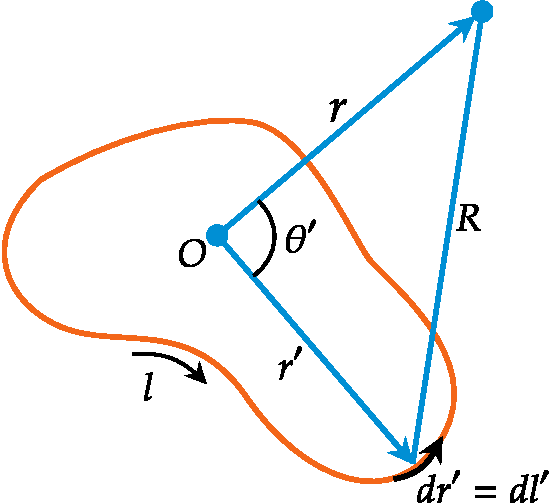
\includegraphics[height=4cm,width=5cm]{diagram-20211216(1)-crop}
	\caption{}
	\label{}
\end{figure}
\begin{align*}
\frac{1}{r}&=\frac{1}{\sqrt{r^{2}+\left(r^{\prime}\right)^{2}-2 r r^{\prime} \cos \theta^{\prime}}}=\frac{1}{r} \sum_{n=0}^{\infty}\left(\frac{r^{\prime}}{r}\right)^{n} P_{n}\left(\cos \theta^{\prime}\right)\\
\text{Accordingly, the vector }&\text{potential of a current loop can be written}\\
\mathbf{A}(\mathbf{r})&=\frac{\mu_{0} I}{4 \pi} \oint \frac{1}{r} d \mathbf{l}^{\prime}=\frac{\mu_{0} I}{4 \pi} \sum_{n=0}^{\infty} \frac{1}{r^{n+1}} \oint\left(r^{\prime}\right)^{n} P_{n}\left(\cos \theta^{\prime}\right) d \mathbf{l}^{\prime},\\
\text{or, more }&\text{explicitly:}\\
\mathbf{A}(\mathbf{r})=& \frac{\mu_{0} I}{4 \pi}\left[\frac{1}{r} \oint d \mathbf{l}^{\prime}+\frac{1}{r^{2}} \oint r^{\prime} \cos \theta^{\prime} d \mathbf{l}^{\prime}\right.\\
&\left.+\frac{1}{r^{3}} \oint\left(r^{\prime}\right)^{2}\left(\frac{3}{2} \cos ^{2} \theta^{\prime}-\frac{1}{2}\right) \dot{d}^{\prime}+\cdots\right]
\end{align*}
 First term represents is called monopole term which doesnt exists.$\left( \oint dl=0\right) $\\
 Second term represents dipole and third term represents quadrapole term.\\
 The main contribution from dipole term can be written as 
 \begin{align*}
 \mathbf{A}_{\mathrm{dip}}(\mathbf{r})&=\frac{\mu_{0} I}{4 \pi r^{2}} \oint r^{\prime} \cos \theta^{\prime} d \mathbf{l}^{\prime}=\frac{\mu_{0} I}{4 \pi r^{2}} \oint\left(\hat{\mathbf{r}} \cdot \mathbf{r}^{\prime}\right) d \mathbf{l}^{\prime}\\
\text{ The integral can }&\text{ be written as}\\
 \oint\left(\hat{\mathbf{r}} \cdot \mathbf{r}^{\prime}\right) d \mathbf{l}^{\prime}&=-\hat{\mathbf{r}} \times \int d \mathbf{a}^{\prime}
\text{ Then }\\
 \mathbf{A}_{\mathrm{dip}}(\mathbf{r})&=\frac{\mu_{0}}{4 \pi} \frac{\mathbf{m} \times \hat{\mathbf{r}}}{r^{2}}\\
\text{ where $\mathbf{m}$ is the }&\text{magnetic dipole moment:}\\
 \mathbf{m} \equiv I \int d \mathbf{a}&=I \mathbf{a} .
 \end{align*}
\section{Magnetic Dipole}
In electrostatics, when two opposite charge placed a small distance apart, it called an electric dipole. Similarly, when a wire carrying a current forms a small closed loop, then it is called magnetic dipole.\\
The magnetic field due to a magnetic dipole is given bellow.Where $B_r$ is the magnetic field at the axial point and $B_{\theta}$ be the magnetic field at point which makes an angle $\theta$ with the axis.
$$\mathbf{B}=\left\{\begin{array}{l}
	B_{r}=2|\boldsymbol{m}| \frac{\mu_{0}}{4 \pi} \frac{\cos \theta}{R^{3}} \\\\
	B_{\theta}=|\boldsymbol{m}| \frac{\mu_{0}}{4 \pi} \frac{\sin \theta}{R^{3}}
\end{array}\right.\hspace{2cm}\text { Where } \boldsymbol{m}=i \mathbf{A} \text { is the magnetic dipole moment of the loop }$$
Here $i$ is the current in the loop, $A$ is the loop area, $R$ is the radial distance from the center of the loop. The field is equivalent to that from a tiny bar magnet (a magnetic dipole).\\
We define \textbf{the magnetic dipole moment to be a vector pointing out of the plane of the current loop and with a magnitude equal to the product of the current and loop area:}
The area vector, and thus the direction of the magnetic dipole moment, is given by a right-hand rule using the direction of the currents.
\begin{center}
	\framebox{
		
		\parbox[t][1.0cm]{4cm}{
			
			\addvspace{0.2cm} \centering 
			Magnetic dipole moment\\
			$m=i A$} 
	}
\end{center}
\begin{note}
	The magnetic field of a dipole can be written in coordinate free form\\
\begin{center}
	\framebox{
		\parbox[t][1.5cm]{3.5cm}{
			
			\addvspace{0.2cm} \centering
			
			\begin{align*}
			\begin{array}{lll}
				B_{dipole}(r)=\frac{\mu_{0}}{4 \pi }\frac{1}{r^3}\left[ 3(m\cdot\hat{r})\hat{r}-m\right]   
			\end{array}
			\end{align*}} }
\end{center}
\end{note}
\subsection{Interaction of Magnetic Dipoles in External Fields }
\subsubsection{Torque}
\begin{minipage}{0.65\textwidth}
	By the $\mathbf{F}=i\ l \times \mathbf{B}_{\text {ext }}$ force law, we know that a current loop (and thus a magnetic dipole) feels a torque when placed in an external magnetic field:
	$$
	\boldsymbol{\tau}=\boldsymbol{m} \times \mathbf{B}_{\text {ext }}
	$$
	The direction of the torque is to line up the dipole moment with the magnetic field.
\end{minipage}
\begin{minipage}{0.35\textwidth}
	\begin{figure}[H]
		\centering
		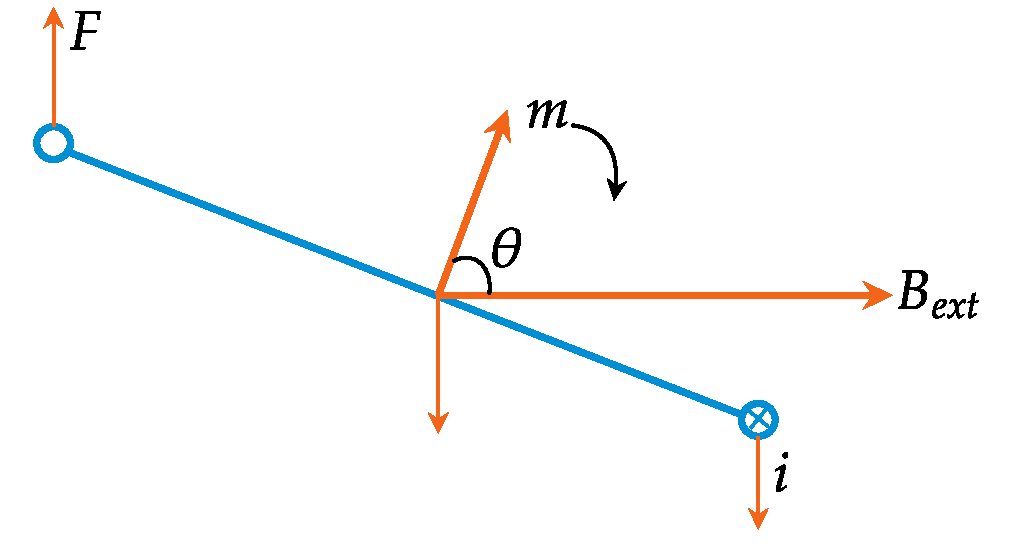
\includegraphics[height=3cm,width=5cm]{magnetic dipole1}
		\caption{Torque on magnetic dipole}
		\label{magnetic dipole1}
	\end{figure}
\end{minipage}
\subsubsection{Potential Energy}
The above equation is analogous to $\vec{\tau}=\overrightarrow{\mathbf{p}} \times \overrightarrow{\mathbf{E}}$ , the torque exerted on an electric dipole moment $\overrightarrow{\mathbf{p}}$ in the presence of an electric field $\overrightarrow{\mathbf{E}}$. Recalling that the potential energy for an electric dipole is $U=-\overrightarrow{\mathbf{p}} \cdot \overrightarrow{\mathbf{E}}$, a similar form is expected for the magnetic case. The work done by an external agent to rotate the magnetic dipole from an angle $\theta_{0}$ to $\theta$ is given by
Let us calculate the work done by the magnetic field when aligning the dipole. Let $\theta$ be the angle between the magnetic dipole direction and the external field direction.\\
\begin{align*}
	W_{\mathrm{ext}} &=\int_{\theta_{0}}^{\theta} \tau d \theta^{\prime}=\int_{\theta_{0}}^{\theta}\left(\mu B \sin \theta^{\prime}\right) d \theta^{\prime}=\mu B\left(\cos \theta_{0}-\cos \theta\right) \\
	&=\Delta U=U-U_{0}
\end{align*}
Once again, $W_{\text {ext }}=-W$, where $W$ is the work done by the magnetic field. Choosing $U_{0}=0$ at $\theta_{0}=\pi / 2$, the dipole in the presence of an external field then has a potential energy of
\begin{align*}
U=-\mu B \cos \theta=-\overrightarrow{\boldsymbol{\mu}} \cdot \overrightarrow{\mathbf{B}}
\end{align*}
The configuration is at a stable equilibrium when $\overrightarrow{\boldsymbol{\mu}}$ is aligned parallel to $\overrightarrow{\mathbf{B}}$, making $U$ a minimum with $U_{\min }=-\mu B$. On the other hand, when $\overrightarrow{\boldsymbol{\mu}}$ and $\overrightarrow{\mathbf{B}}$ are anti-parallel, $U_{\max }=+\mu \mathrm{B}$ is a maximum and the system is unstable.
\begin{center}
	\framebox{
		
		\parbox[t][3.0cm]{10cm}{
			
			\addvspace{0.2cm} \centering 
			\begin{alignat*}{2}
				&\text{Magnetic Moment of Current Carrying Wire:}  &&\overrightarrow{\boldsymbol{\mu}}=I \overrightarrow{\mathbf{A}} \\&\text{Torque on Magnetic Moment:}
			&&\overrightarrow{\mathbf{\tau}}=\overrightarrow{\boldsymbol{\mu}} \times \overrightarrow{\mathbf{B}}
			\\&\text{Energy of Moment in External Field:}
			&&U=-\overrightarrow{\boldsymbol{\mu}} \cdot \overrightarrow{\mathbf{B}}
			\end{alignat*}
		 
	}}
\end{center}
\subsection{The interaction energy of two magnetic dipoles}
The interaction energy of two magnetic dipoles seperated by a displacement r is given by\\
\begin{center}
	\framebox{
		\parbox[t][1.3cm]{3.5cm}{
			
			\addvspace{0.2cm} \centering
			
			\begin{align*}
			\begin{array}{lll}
			U=\frac{\mu_{0}}{4\pi}\frac{1}{r^3}\left[ m_1 \cdot m_2-3(m\cdot \hat{r})(m_2 \cdot \hat{r})\right]  
			\end{array}
			\end{align*}} }
\end{center} 
\subsection{Torque On Current Loop}
	\begin{figure}[H]
	\begin{center}
		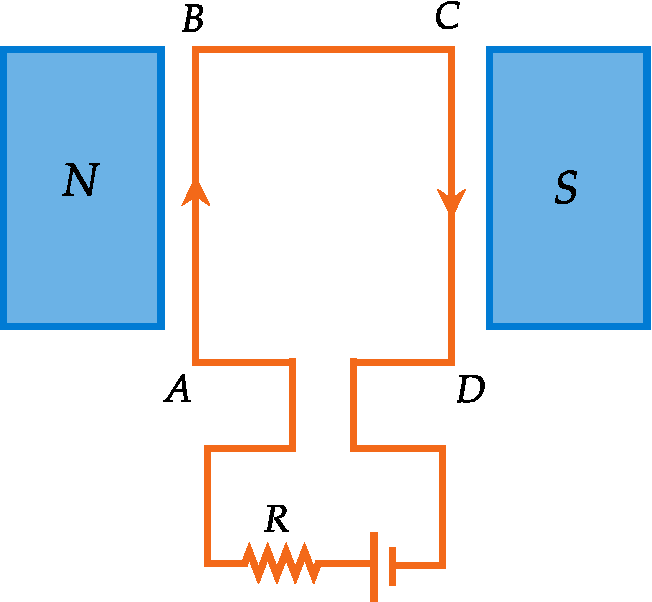
\includegraphics[width=0.25\textwidth]{torque}
	\end{center}
\end{figure}
Let us now consider the case when the magnetic field $B$ is in the plane with the rectangular loop. No force is exerted by the field on the arms of the loop that is parallel to the magnets, but the arms perpendicular to the magnets experience a force given by $F_{1}$
\begin{align*}
F_{1}&=I b B
\intertext{This force is directed into the plane.
Similarly, we can write the expression for a force $\mathrm{F}_{2}$ which is exerted on the arm CD,}
F_{2}&=I b B=F_{1}\\
\text{We see that the net force on the }&\text{loop is zero and the torque on the loop is given by,}\\
\tau&=F_{1} \frac{a}{2}+F_{2} \frac{a}{2} \\
\tau&=I b B \frac{a}{2}+I b B \frac{a}{2}=I(a b) B=I A B
\end{align*}
Where ab is the area of the rectangle. Here, the torque tends to rotate the loop in the anti-clockwise direction. Let us consider the case when the plane of the loop is not along the magnetic field. Let the angle between the field and the normal to the coil be given by $\theta$. We can see that the forces on the arms BC and DA will always act opposite to each other and will be equal in magnitude. Since these forces are the equal opposite and collinear at all points, they cancel out each other's effect and this results in zero-force or torque. The forces on the arms $A B$ and $\mathrm{CD}$ are given by $\mathrm{F}_{1}$ and $\mathrm{F}_{2}$. These forces are equal in magnitude and opposite in direction and can be given by,\\
These forces are not collinear and thus act as a couple exerting a torque on the coil. The magnitude of the torque can be given by,
$$
\begin{aligned}
F_{1}&=F_{2}=I b B
\tau&=F_{1} \frac{a}{2} \sin \theta+F_{2} \frac{a}{2} \sin \theta \\
\tau&=I a b B \sin \theta \\
\tau&=I A B \sin \theta
\end{aligned}
$$
\section{Motion of charged particle in Electric and magnetic Field}
\subsection{Motion of charged particle in uniform magnetic field}
\textbf{(a)}\quad \textbf{If the particle enters $\perp^r$ to the field\quad(Circular)}\\\\
When the particle of charge $\theta$\ enters $\perp^r$\ to the field, if under go circular motion and the centripetal acceleration is provided by magnetic force $qVB$. If it moves in a circular path of radius $R$,\\
\begin{minipage}{0.65\textwidth}
	\begin{align*}
	QVB&=\frac{mv^2}{R}\quad \Rrightarrow\quad\text{ Cyclotron formula.}\\
	R&=\frac{mv}{QB},\quad m \ \text{Is the man of the particle}\\
	\text{When $R$ is the}&\text{ cyclotron radius.}\\
	\text{Momentum}\ P&=mv=\frac{m\times QBR}{m}\\
	&=QBR\\
	\text{Kinetic energy}\ KE&=\frac{P^2}{2m}=\frac{\theta^2B^2R^2}{2m}\\
	\text{Time period }\ T&=\frac{2\pi R}{V}=\frac{2\pi m}{\theta B}
	\end{align*}
\end{minipage}
	\begin{minipage}{0.35\textwidth}
	\begin{figure}[H]
		\centering
		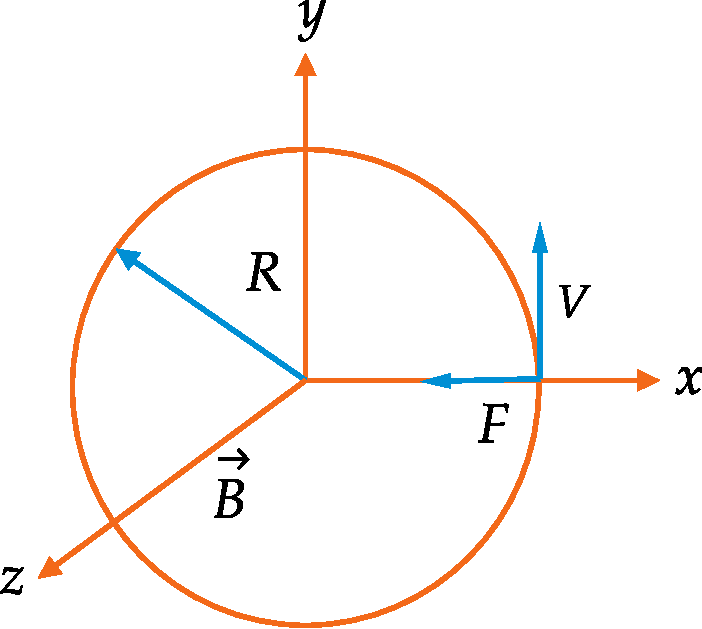
\includegraphics[height=4cm,width=4.5cm]{diagram-20210427(4)-crop}
		\caption{Circular path of the particle entering perpendicular to the magnetic field}
		\label{Cyclotron}
	\end{figure}				
\end{minipage}
\textbf{(b)}\quad \textbf{The Ratio of Various Quantities}\\
\begin{enumerate}
	\item $\frac{r_1}{r_{2}}=\frac{q_{2}}{q_{1}} \sqrt{\frac{m_{1}}{m_{2}}}$, when $E_{K}$ and $B$ are constants.
\item $\frac{r_{1}}{r_{2}}=\frac{q_{2}}{q_{1}} \sqrt{\frac{m_{1} E_{K_{1}}}{m_{2} E_{K_{2}}}}$, when $B$ is constant.
\item  $\frac{p_{1}}{p_{2}}=\frac{q_{1}}{q_{2}}\left(\frac{r_{1}}{r_{2}}\right)$
\item $\frac{\omega_{1}}{\omega_{2}}=\frac{q_{1} m_{2}}{q_{2} m_{1}}=\frac{v_{1}}{v_{2}}$
\item $\frac{T_{1}}{T_{2}}=\frac{q_{2}}{q_{1}} \times \frac{m_{1}}{m_{2}}$\\
\item  $\frac{E_{K_{l}}}{E_{K_{2}}}=\frac{q_{1}^{2} r_{1}^{2}}{q_{2}^{2} r_{2}^{2}} \times \frac{m_{2}}{m_{1}}$
\end{enumerate}
\textbf{(c)}\quad \textbf{If the particle enters the field with an angle making $\theta$with it helical motion}\\\\
When it enters with an angle $\theta$ with the field $n$ has two component,\quad $V_\parallel=V \cos\theta$\quad and \quad$V_\perp^r=V\sin\theta$\\No magnetic force along parallel direction here again\\
\begin{minipage}{0.65\textwidth}
	\begin{align*}
	R&=\frac{MV_\perp r}{QB} =\frac{MV \sin\theta}{QB}\\
	T&=\frac{2\pi m}{QB}\quad \text{has no change}
	\intertext{Due to parallel component of velocity, particle undergo helical motion. Horizontal distance travelled by the particle during one period of revolution is called Pitch,}
	D&=T\times V cos \theta\\
	b&=\frac{2\pi m}{QB} V \cos \theta 
	\end{align*}
\end{minipage}
\begin{minipage}{0.35\textwidth}
	\begin{figure}[H]
		\centering
		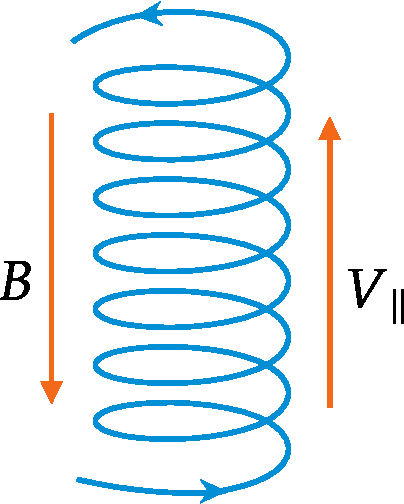
\includegraphics[height=3cm,width=3.5cm]{diagram-20210427(6)-crop}
		\caption{Helical path of the particle entering at an angle to the magnetic field}
		\label{Helical path of the particle }
	\end{figure}
\end{minipage}
\subsection{Motion of charged particle in static electric field.}
\textbf{(a)}\quad Charged particle enters in the direction of field (Linear motion)
\begin{align*}
\intertext{If $q$ charged moves in uniform field then,}
F&=q E \hspace{2cm} F=\frac{md^2r}{dt^2}\\
\frac{md^2r}{dt^2}&=qE\\
\frac{dr}{dt}&=\frac{qEt}{m}+C_0\\
\text{At} \quad t=0\quad V&=V_0,\quad \text{and}\quad r=r_0,\\
\text{Then}\quad c_0&=V_0\\
\frac{d_0}{dt}&=\frac{qE}{m}t+V_0\\
r&=\frac{qEt^2}{2m}+V_0t+r_0
\end{align*} 
 \begin{minipage}{0.65\textwidth}
 	\begin{align*}
 	\intertext{It initial position and velocity are zeros,}
 	\text{Then}\quad V&=\frac{Q E}{m}t\\
 	r&=\frac{Q E}{2m}t^2
 \end{align*} 	
 	\end{minipage}
 \begin{minipage}{0.35\textwidth}
 	\begin{figure}[H]
 		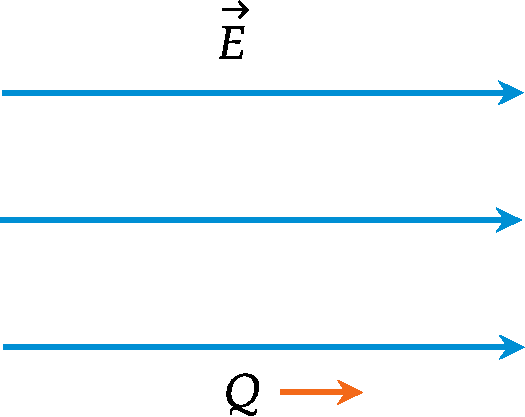
\includegraphics[height=3cm,width=4cm]{diagram-20210427(11)-crop}
 		\caption{Linear motion of charged particle in Static electric field.}
 		\label{Linear motion of charged particle}
 	\end{figure}
 \end{minipage}
\begin{align*}
\text{Energy acquired by the  }&\text{charged particle moving from initial to some final point,}\\
w&=\int f\cdot dl=m\int_{V_1}^{V_2}a\cdot dl\\
&=m\int_{V_1}^{V_2}\frac{dV}{dt}\times Vdt=m\int_{1}^{2}VdV=\frac{1}{2}m(V^2_2-V^2_1)\\
w&=\frac{1}{2}m(V^2_2-V^2_1)\\
\text{If initial velocity }V_1&=0\\
w&=\frac{1}{2}mV^2\\
\text{If the potential difference }&\text{between them is $V$ then,}\\
w&=QV=\frac{1}{2}mV^2\\
\therefore V&=\sqrt{\frac{2QV}{m}}\\
K.E&=w=\frac{1}{2}m\times\frac{Q^2 E^2}{m^2}t^2\\
&=QE\times\frac{QE}{2m}t^2\\
&=QEr
\end{align*}
\textbf{(b)}\quad \textbf{Charged particle enters in the direction $\perp^r$ to the electric field (Parabolic motion)}\\
 \begin{minipage}{0.55\textwidth}
Let us consider a charge particle enters in a electric field region with velocity $V_x$ at\ $t=0$. The electric field is in $y$ direction and the field region has length $l$. After traversing a distance $l$ it strikes a point $P$ on a screen which is placed at a distance $L$ from the field region. \\
Since electric field is in the $y$ direction , charged particle will experience force.
\begin{align*}
F_y&=QEy\\ 
\intertext{Acceleration}
a_y&=\frac{QEy}{m}\\
\end{align*}
\end{minipage}
\begin{minipage}{0.45\textwidth}
	\begin{figure}[H]
		\centering
		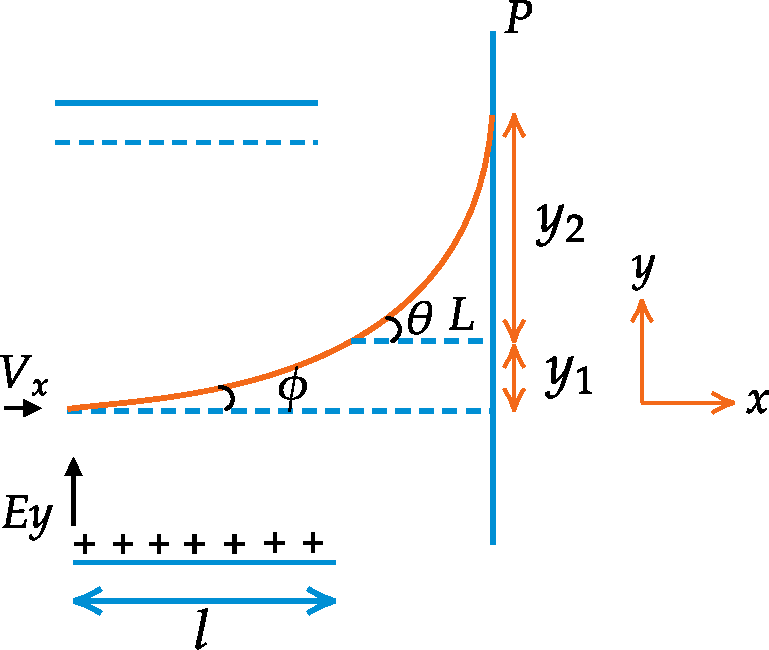
\includegraphics[height=4.5cm,width=6cm]{diagram-20210427(5)-crop}
		\caption{Parabolic motion of Charged particle entering in   perpendicular direction to the electric field.}
		\label{rc current discharge}
	\end{figure}
\end{minipage}\\\\	
In time $t$ , charge particle will traverse a distance $y=\frac{1}{2}a_yt^2$ in $y$ direction and a distance $x=V_xt$\  in$x$ direction.
\begin{align*}
\text{Thus}\quad y=\frac{1}{2}a_yt^2&=\frac{QEy}{2m}(\frac{x}{V_x})^2 \quad\text{represents a parabola}\\
y_1&=\frac{QEy}{2m}(\frac{l}{V_x})^2\text{and}\quad y_2=L \tan\theta\\
\text{Thus distance of point $P$}&\text{ from the center of the screen is}\\
y_1+y_2&=\frac{QEy}{2m}(\frac{l}{V_x})^2+L \tan\theta\\
\text{Angle of deviation in the }&\text{field region}\\
\tan\phi&=\frac{dy}{dx}=\frac{QEy}{mV_x^2}x\\
\text{Angle of deviation in the field }&\text{foce  region}\\
\tan\theta&=\frac{QEy}{mV_x^2}l
\end{align*}
\subsection{Charged particle in uniform electric and magnetic field }
\textbf{(a)}\quad \textbf{$E$ and $B$ are perpendicular(Cycloid motion).}\\
\begin{minipage}{0.65\textwidth}
		If $B$ points in $\hat{x}$ direction $E$ in the $z$ direction. Suppose the particle is at origin initially. So $F_{mg} =0$, due $E$ it moves along $\hat{z} $ direction, When it starts moving magnetic force develop, it pulls the charge to right, when $V$ increases $F_{mg} $ increases ,it tend to move in a circular path,which results the particle move back towards $Y$ axis at that time it is moving against $\vec{E}$. Therefore the velocity  $V$ decreases, and $F_{mag} $ also decreases. Then $E$ bring the charge to rest at point $a$. Then  the entire process repeats.
\end{minipage}
\begin{minipage}{0.35\textwidth}
	\begin{figure}[H]
		\centering
		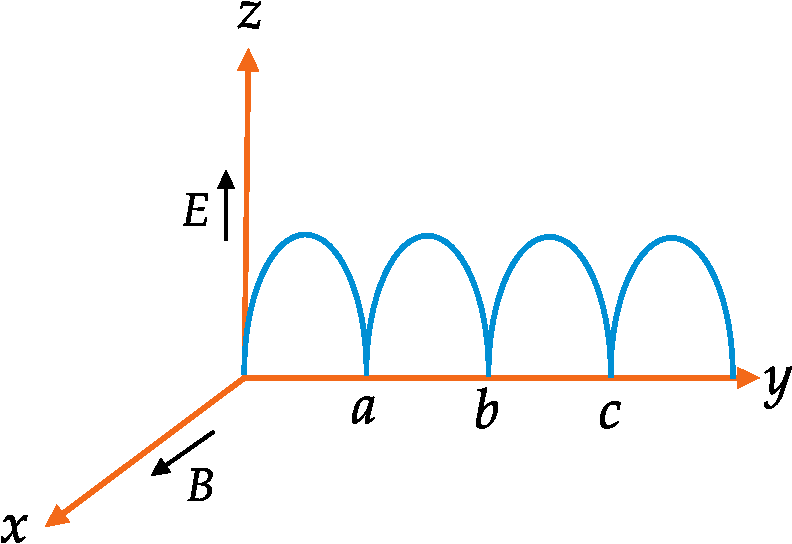
\includegraphics[height=3cm,width=5cm]{diagram-20210427(8)-crop}
		\caption{Cycloid motion of charge}
		\label{cycloid }
	\end{figure}
\end{minipage}
\begin{align*}
\text{We know particle is at rest at}&\text{ origin when time $t=0$ ,Then,} \\
y(0)&=z(0)=0\\
\dot{y}(0)&=\dot{z}(0)=0\quad\text{No motion along $x$ axis}\\
V&=(0,\dot{y},\dot{z})\\
V\times B&=\left|\begin{array}{lll}\hat{x} & \hat{y}&\hat{z} \\ 0 & \dot{y}&\dot{z} \\B & 0&0\end{array}\right|=B\dot{z}\hat{y}-B\dot{y}\hat{z}\\
\text{Total force}\ F&=Q[E+V\times B]=Q[E\hat{z}+B\dot{z}\hat{y}-B\dot{y}\hat{z}]\\
ma&=m[\dot{y}\hat{y}+\dot{z}\hat{z}]\\
m[\dot{y}\hat{y}+\dot{z}\hat{z}]&=Q[E\hat{z}+B\dot{z}\hat{y}-B\dot{y}\hat{z}]\\
\text{Comparing the coefficient }&\text{ $ \hat{y} $ and $ \hat{z} $}\\
QB\dot{z}&=m\dot{y}\hspace{1cm}E-QB\dot{y}=m\dot{z}\\
\text{let}\quad w&=\frac{QB}{m},\quad \text{Cyclotron frequency in absence of $\vec{E}$}\\
\text{Then}, \dot{y}&=w\dot{z},\quad \dot{z}=w\left( \frac{E}{B}-\dot{y}\right)\\ 
\text{Their Solution,}\\
y(t)&=c_1\cos wt+c_2\sin wt+\left( \frac{E}{B}\right) t+c_3\\
z(t)&=c_2\cos wt-c_1\sin wt+c_4\\
\text{Applying the initial  conditions}&\text{ we will get $ c_1,c_2,c_3.c_4 $}\\
y(t)&=\frac{E}{wB}(wt-\sin wt)\\
z(t)&=\frac{E}{wB}(1-\cos wt)\\
\text{Now let}\quad R&=\frac{E}{wB}\\
\text{and using }\sin^2wt+&\cos^2wt=1\\
\text{We will get}\quad (y-Rwt)^2&+(z-R)^2=R^2\\
\text{Which represents the formula of a }&\text{circle whose center $(0,Rwt,R)$ travels in $y$ direction at speed.}\\
 V&=wR=\frac{E}{B}\\
\text{curve generated by this motion is }&\text{called cycloid.}
\end{align*}
\textbf{(b)}\quad \textbf{When $E$ and $B$ are parallel}\\
The particle will move in helical path of constant radius but varying pitch.
\begin{figure}[H]
			\centering
		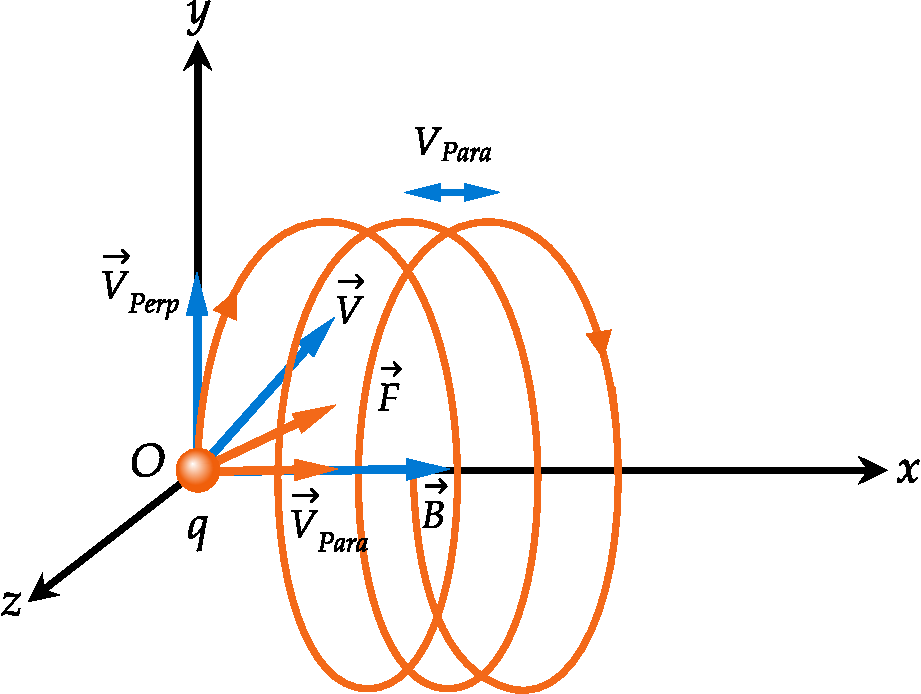
\includegraphics[height=4cm,width=6cm]{helical}
		\caption{Helical path of charged particle in Electric and magnetic field}
		\label{Helical path}
	\end{figure}

	
	
\begin{exercise}
	A neutron, a proton, an electron and an $\alpha$particle enter a region of constant magnetic field with equal velocities. The magnetic field is inward normal to the plane of paper. Label the tracks of the particle?\\
	\begin{minipage}{.45\textwidth}
		\begin{center}
			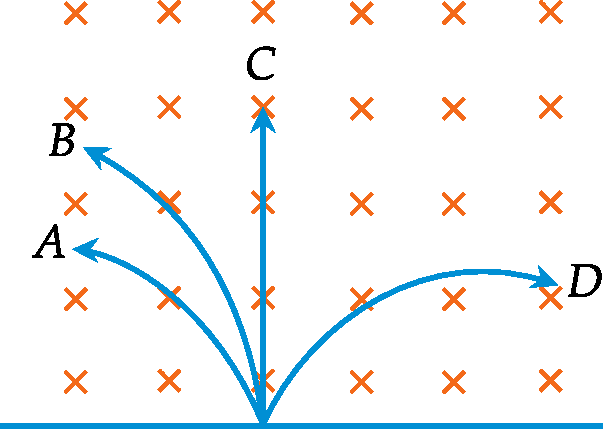
\includegraphics[width=0.5\textwidth]{diagram-20210427(9)-crop}
		\end{center}
	\end{minipage}
\end{exercise}
\begin{answer}
	Since neutron has no charge it is undeflected by the field. So it is represented by $C$ . So all particle has initial velocity along $C$ and force $( \theta(V\times B))$pointed towards left for $+ve$ particles and right for electron. And radius is directly proportional to $m$,so $\alpha$particle have larger radius. So,\\\\
	A=proton\quad B)$\rightarrow$$\alpha$particle\quad C)$\rightarrow$neutron\quad D)$\rightarrow$electron.
\end{answer}
\begin{exercise}
	A particle having a charge $a$ and mass $m$ moves along a circle of radius $R$ under the action of magnetic field $B$. When the particle is at a point $P$, a uniform electric field is switched on and it is found that the particle continues on the tangent through $P$ with a uniform velocity. The magnitude of electric field is,?
\end{exercise}
\begin{answer}
	\begin{align*}
	Q E&=\theta VB\\
	E&=VB\\
	\text{Where $V$ is the }&\text{velocity }\\
	 V&=\frac{\theta BR}{m}\\
	\therefore E&=\frac{QB^2R}{m}
	\end{align*}
\end{answer}
\begin{exercise}
	A particle of mass carrying charge q is moving in a circle in a magnetic field.According to Bohr's model, Find?\\
	(a) The radius of the particle in the nth level.\\
	(bThe energy of the particle in the nth level
\end{exercise}
\begin{answer}
\begin{align*}
(a)mv_nr_n&=n\bar{h} \quad r_n=\frac{mv_n}{qB}\\
r_n&=\frac{m}{qB}\frac{n\bar{h}}{mv_n}\\
r_n^2&=\frac{n\bar{h}}{qB}\\
r_n&=\sqrt{\frac{n\bar{h}}{qB}}\\
(b) E_n&=\frac{q^2B^2r^2_n}{2m}\implies \frac{q^2B^2}{2m}\times\frac{n\bar{h}}{qB}=n\left( \frac{qBh}{4\pi m}\right)  
\end{align*}
\end{answer}
\newpage
\begin{abox}
	Practice set 1
	\end{abox}
\begin{enumerate}
\begin{minipage}{\textwidth}
	\item The magnetic field at a distance $R$ from a long straight wire carrying a steady current $I$ is proportional to
	\exyear{NET 2012}
\end{minipage}
\begin{tasks}(4)
	\task[\textbf{A.}] $I R$
	\task[\textbf{B.}] $I / R^{2}$
	\task[\textbf{C.}]$I^{2} / R^{2}$
	\task[\textbf{D.}]$I / R$
\end{tasks}
\begin{minipage}{\textwidth}
	\item The vector potential $\vec{A}$ due to a magnetic moment $\vec{m}$ at a point $\vec{r}$ is given by $\vec{A}=\frac{\vec{m} \times \vec{r}}{r^{3}}$.
	If $\vec{m}$ is directed along the positive $z$-axis, the $x$ - component of the magnetic field, at the point $\vec{r}$, is
	\exyear{NET 2011}
\end{minipage}
\begin{tasks}(4)
	\task[\textbf{A.}] $\frac{3 m y z}{r^{5}}$
	\task[\textbf{B.}] $-\frac{3 m x y}{r^{5}}$
	\task[\textbf{C.}]$\frac{3 m x z}{r^{5}}$
	\task[\textbf{D.}]$\frac{3 m\left(z^{2}-x y\right)}{r^{5}}$
\end{tasks}
\begin{minipage}{\textwidth}
	\item An infinite solenoid with its axis of symmetry along the $z$-direction carries a steady current $I$.
	The vector potential $\vec{A}$ at a distance $R$ from the axis
	\exyear{NET 2012}
	\begin{figure}[H]
		\centering
		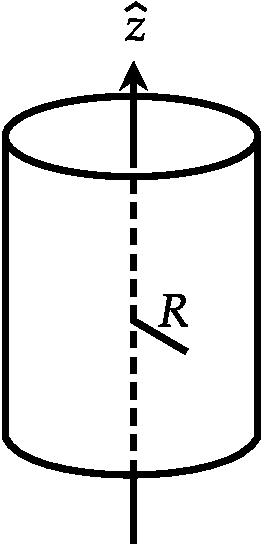
\includegraphics[height=3.5cm,width=2cm]{NET1}
	\end{figure}
\end{minipage}
\begin{tasks}(1)
	\task[\textbf{A.}]Is constant inside and varies as $R$ outside the solenoid
	\task[\textbf{B.}]Varies as $R$ inside and is constant outside the solenoid
	\task[\textbf{C.}]Varies as $\frac{1}{R}$ inside and as $R$ outside the solenoid
	\task[\textbf{D.}]Varies as $R$ inside and as $\frac{1}{R}$ outside the solenoid
\end{tasks}
\begin{minipage}{\textwidth}
	\item The force between two long and parallel wires carrying currents $I_{1}$ and $I_{2}$ and separated by a distance $D$ is proportional to
	\exyear{NET 2013}
\end{minipage}
\begin{tasks}(4)
	\task[\textbf{A.}] $I_{1} I_{2} / D$
	\task[\textbf{B.}]$\left(I_{1}+I_{2}\right) / D$
	\task[\textbf{C.}]$\left(I_{1} I_{2} / D\right)^{2}$
	\task[\textbf{D.}]$I_{1} I_{2} / D^{2}$
\end{tasks}
\begin{minipage}{\textwidth}
	\item A time-dependent current $\vec{I}(t)=K t \hat{z}$ (where $K$ is a constant) is switched on at $t=0$ in an infinite current-carrying wire. The magnetic vector potential at a perpendicular distance $a$ from the wire is given (for time $t>a / c$ ) by
	\exyear{NET 2014}
\end{minipage}
\begin{tasks}(2)
	\task[\textbf{A.}] $\hat{z} \frac{\mu_{0} K}{4 \pi c} \int_{-\sqrt{c^{2} t^{2}-a^{2}}}^{\sqrt{c^{2} t^{2}-a^{2}}} d z \frac{c t-\sqrt{a^{2}+z^{2}}}{\left(a^{2}+z^{2}\right)^{1 / 2}}$
	\task[\textbf{B.}] $\hat{z} \frac{\mu_{0} K}{4 \pi} \int_{-c t}^{c t} d z \frac{t}{\left(a^{2}+z^{2}\right)^{1 / 2}}$
	\task[\textbf{C.}] $\hat{z} \frac{\mu_{0} K}{4 \pi c} \int_{-c t}^{c t} d z \frac{c t-\sqrt{a^{2}+z^{2}}}{\left(a^{2}+z^{2}\right)^{1 / 2}}$
	\task[\textbf{D.}] $\hat{z} \frac{\mu_{0} K}{4 \pi} \int_{-\sqrt{c^{2} t^{2}-a^{2}}}^{\sqrt{c^{2} t^{2}-a^{2}}} d z \frac{t}{\left(a^{2}+z^{2}\right)^{1 / 2}}$
\end{tasks}
\begin{minipage}{\textwidth}
	\item A charged particle moves in a helical path under the influence of a constant magnetic field. The initial velocity is such that the component along the magnetic field is twice the component in the plane normal to the magnetic field.
	The ratio $\ell / R$ of the pitch $\ell$ to the radius $R$ of the helical path is
	\exyear{NET 2014}
\end{minipage}
\begin{tasks}(4)
	\task[\textbf{A.}] $\pi / 2$
	\task[\textbf{B.}]$4 \pi$
	\task[\textbf{C.}]$2 \pi$
	\task[\textbf{D.}]$\pi$
\end{tasks}
\begin{minipage}{\textwidth}
	\item A proton moves with a speed of $300 \mathrm{~m} / \mathrm{s}$ in a circular orbit in the $x y$-plan in a magnetic field 1 tesla along the positive $z$-direction. When an electric field of $1 \mathrm{~V} / \mathrm{m}$ is applied along the positive $y$-direction, the center of the circular orbit
	\exyear{NET 2014}
\end{minipage}
\begin{tasks}(1)
	\task[\textbf{A.}]Remains stationary
	\task[\textbf{B.}]Moves at $1 \mathrm{~m} / \mathrm{s}$ along the negative $x$-direction
	\task[\textbf{C.}]Moves at $1 \mathrm{~m} / \mathrm{s}$ along the positive $z$ - direction
	\task[\textbf{D.}]Moves at $1 \mathrm{~m} / \mathrm{s}$ along the positive $x$ - direction
\end{tasks}
\begin{minipage}{\textwidth}
	\item Given a uniform magnetic field $B=B_{0} \hat{k}$ (where $B_{0}$ is a constant), a possible choice for the magnetic vector potential $A$ is
	\exyear{NET 2015}
\end{minipage}
\begin{tasks}(4)
	\task[\textbf{A.}] $B_{0} y \hat{i}$
	\task[\textbf{B.}] $-B_{0} y \hat{i}$
	\task[\textbf{C.}] $B_{0}(x \hat{j}+y \hat{i})$
	\task[\textbf{D.}]$B_{0}(x \hat{i}+y \hat{j})$
\end{tasks}
\begin{minipage}{\textwidth}
	\item A small magnetic needle is kept at $(0,0)$ with its moment along the $x$-axis. Another small magnetic needle is at the point $(1,1)$ and is free to rotate in the $x y$ - plane. In equilibrium the angle $\theta$ between their magnetic moments is such that
	\exyear{NET 2015}
\end{minipage}
\begin{tasks}(4)
	\task[\textbf{A.}] $\tan \theta=\frac{1}{3}$
	\task[\textbf{B.}]$\tan \theta=0$
	\task[\textbf{C.}]$\tan \theta=3$
	\task[\textbf{D.}]$\tan \theta=1$
\end{tasks}
\begin{minipage}{\textwidth}
	\item A dipole of moment $\vec{p}$, oscillating at frequency $\omega$, radiates spherical waves. The vector potential at large distance is\\
	$$\vec{A}(\vec{r})=\frac{\mu_{0}}{4 \pi} i \omega \frac{e^{i k r}}{r} \vec{p}$$	
	$\text { To order }\left(\frac{1}{r}\right) \text { the magnetic field } \vec{B} \text { at a point } \vec{r}=r \hat{n} \text { is }$
	\exyear{NET 2015}
\end{minipage}
\begin{tasks}(2)
	\task[\textbf{A.}] $-\frac{\mu_{0}}{4 \pi} \frac{\omega^{2}}{C}(\hat{n} \cdot \vec{p}) \hat{n} \frac{e^{i k r}}{r}$
	\task[\textbf{B.}]$-\frac{\mu_{0}}{4 \pi} \frac{\omega^{2}}{C}(\hat{n} \times \vec{p}) \frac{e^{i k r}}{r}$
	\task[\textbf{C.}]$-\frac{\mu_{0}}{4 \pi} \omega^{2} k(\hat{n} \cdot \vec{p}) \vec{p} \frac{e^{i k r}}{r}$
	\task[\textbf{D.}]$-\frac{\pi_{0}}{4 \pi} \frac{\omega^{2}}{C} \vec{p} \frac{e^{i k r}}{r}$
\end{tasks}
\begin{minipage}{\textwidth}
	\item A loop of radius $a$, carrying a current $I$, is placed in a uniform magnetic field $B$. If the normal to the loop is denoted by $\hat{n}$, the force $\vec{F}$ and the torque $\vec{T}$ on the loop are
	\exyear{NET 2015}
\end{minipage}
\begin{tasks}(2)
	\task[\textbf{A.}] $\vec{F}=0$ and $\vec{T}=\pi a^{2} I \hat{\mathrm{n}} \times B$
	\task[\textbf{B.}]$\vec{F}=\frac{\mu_{0}}{4 \pi} \vec{I} \times \vec{B}$
	\task[\textbf{C.}]$\vec{F}=\frac{\mu_{0}}{4 \pi} \vec{I} \times \vec{B}$ and $\vec{T}=I \hat{\mathrm{n}} \times \vec{B}$
	\task[\textbf{D.}]$\vec{F}=0$ and $\vec{T}=\frac{1}{\mu_{0} \varepsilon_{0}} I \vec{B}$
\end{tasks}
\begin{minipage}{\textwidth}
	\item A conducting circular disc of radius $r$ and resistivity $\rho$ rotates with an angular velocity $\omega$ in a magnetic field $B$ perpendicular to it. A voltmeter is connected as shown in the figure below. Assuming its internal resistance to be infinite, the reading on the voltmeter
	\exyear{NET 2016}
	\begin{figure}[H]
		\centering
		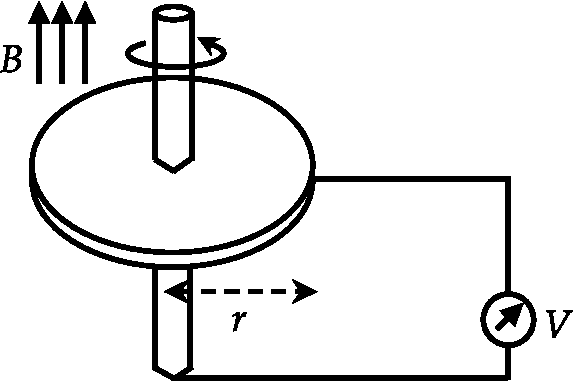
\includegraphics[height=3cm,width=4.5cm]{diagram-20211011(46)-crop}
	\end{figure}
\end{minipage}
\begin{tasks}(1)
	\task[\textbf{A.}] Depends on $\omega, B, r$ and $\rho$
	\task[\textbf{B.}]Depends on $\omega, B$ and $r$ but not on $\rho$
	\task[\textbf{C.}]Is zero because the flux through the loop is not changing
	\task[\textbf{D.}]Is zero because a current the flows in the direction of $B$
\end{tasks}
\begin{minipage}{\textwidth}
	\item A set of $N$ concentric circular loops of wire, each carrying a steady current $I$ in the same direction, is arranged in a plane. The radius of the first loop is $r_{1}=a$ and the radius of the $n^{\text {th }}$ loop is given by $r_{n}=n r_{n-1}$. The magnitude $B$ of the magnetic field at the centre of the circles in the limit $N \rightarrow \infty$, is
	\exyear{NET 2016}
\end{minipage}
\begin{tasks}(2)
	\task[\textbf{A.}] $\mu_{0} I\left(e^{2}-1\right) / 4 \pi a$
	\task[\textbf{B.}]$\mu_{0} I(e-1) / \pi a$
	\task[\textbf{C.}]$\mu_{0} I\left(e^{2}-1\right) / 8 a$
	\task[\textbf{D.}]$\mu_{0} I(e-1) / 2 a$
\end{tasks}
\begin{minipage}{\textwidth}
	\item A constant current $I$ is flowing in a piece of wire that is bent into a loop as shown in the figure.\\
	\begin{figure}[H]
		\centering
		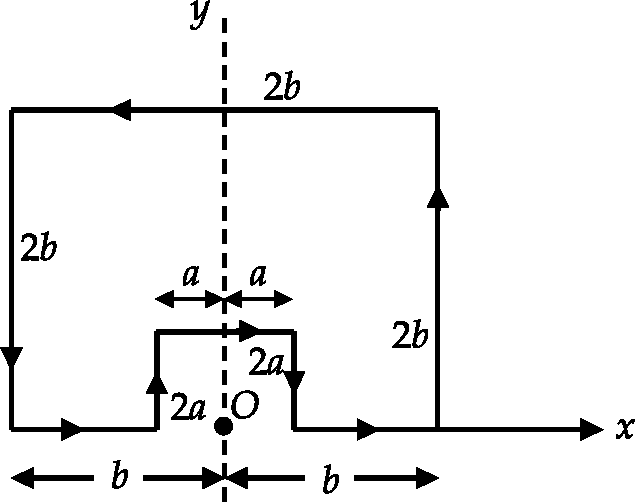
\includegraphics[height=5cm,width=7cm]{diagram-20211011(54)-crop}
	\end{figure}
	$\text { The magnitude of the magnetic field at the point } O \text { is }$
	\exyear{NET 2017}
\end{minipage}
\begin{tasks}(4)
	\task[\textbf{A.}] $\frac{\mu_{0} I}{4 \pi \sqrt{5}} \ln \left(\frac{a}{b}\right)$
	\task[\textbf{B.}]$\frac{\mu_{0} I}{4 \pi \sqrt{5}}\left(\frac{1}{a}-\frac{1}{b}\right)$
	\task[\textbf{C.}]$\frac{\mu_{0} I}{4 \pi \sqrt{5}}\left(\frac{1}{a}\right)$
	\task[\textbf{D.}]$\frac{\mu_{0} I}{4 \pi \sqrt{5}}\left(\frac{1}{b}\right)$
\end{tasks}
\begin{minipage}{\textwidth}
	\item A circular current carrying loop of radius $a$ carries a steady current. A constant electric charge is kept at the centre of the loop. The electric and magnetic fields, $\vec{E}$ and $\vec{B}$ respectively, at a distance $d$ vertically above the centre of the loop satisfy
	\exyear{NET 2017}
\end{minipage}
\begin{tasks}(4)
	\task[\textbf{A.}] $\vec{E} \perp \vec{B}$
	\task[\textbf{B.}] $\vec{E}=0$
	\task[\textbf{C.}]$\vec{\nabla}(\vec{E} \cdot \vec{B})=0$
	\task[\textbf{D.}]$\vec{\nabla} \cdot(\vec{E} \times \vec{B})=0$
\end{tasks}
\begin{minipage}{\textwidth}
	\item \text { The loop shown in the figure below carries a steady current } I \\
	\begin{figure}[H]
		\centering
		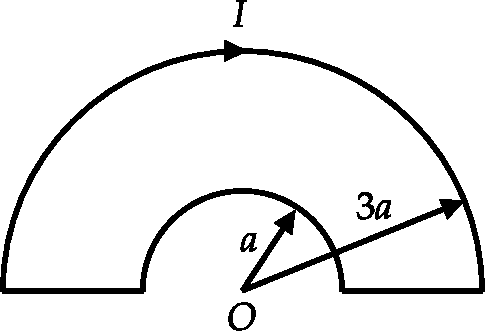
\includegraphics[height=3cm,width=5cm]{diagram-20211011(11)-crop}
	\end{figure}
	$\text { The magnitude of the magnetic field at the point } O \text { is }$
	\exyear{NET 2018}
\end{minipage}
\begin{tasks}(4)
	\task[\textbf{A.}] $\frac{\mu_{0} I}{2 a}$
	\task[\textbf{B.}]$\frac{\mu_{0} I}{6 a}$
	\task[\textbf{C.}]$\frac{\mu_{0} I}{4 a}$
	\task[\textbf{D.}]$\frac{\mu_{0} I}{3 a}$
\end{tasks}
\begin{minipage}{\textwidth}
	\item Two current-carrying circular loops, each of radius $R$, are placed perpendicular to each other, as shown in the figure.
	
	The loop in the $x y$ - plane carries a current $I_{0}$ while that in the $x z$-plane carries a current $2 I_{0}$. The resulting magnetic field $\vec{B}$ at the origin is
	\exyear{NET 2018 dec}
	\begin{figure}[H]
		\centering
		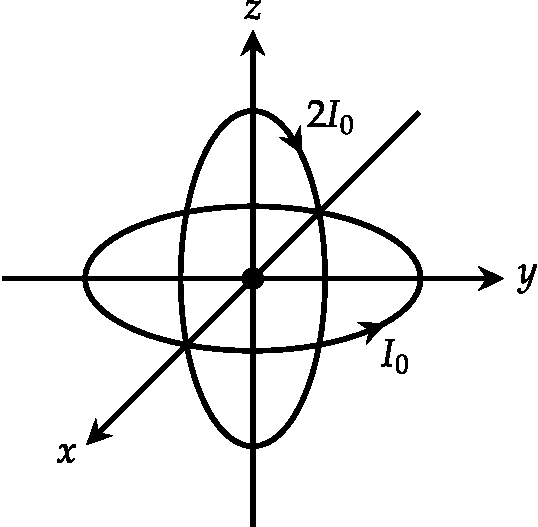
\includegraphics[height=3.5cm,width=5cm]{diagram-20211011(12)-crop}
	\end{figure}
\end{minipage}
\begin{tasks}(2)
	\task[\textbf{A.}] $\frac{\mu_{0} l_{0}}{2 R}[2 \hat{j}+\hat{k}]$ 
	\task[\textbf{B.}]$\frac{\mu_{0} l_{0}}{2 R}[2 \hat{j}-\hat{k}]$
	\task[\textbf{C.}]$\frac{\mu_{0} l_{0}}{2 R}[-2 \hat{j}+\hat{k}]$
	\task[\textbf{D.}]$\frac{\mu_{0} l_{0}}{2 R}[-2 \hat{j}-\hat{k}]$
\end{tasks}
\end{enumerate}
\colorlet{ocre1}{ocre!70!}
\colorlet{ocrel}{ocre!30!}
\setlength\arrayrulewidth{1pt}
\begin{table}[H]
	\centering
	\arrayrulecolor{ocre}
	
	\begin{tabular}{|p{1.5cm}|p{1.5cm}||p{1.5cm}|p{1.5cm}|}
		\hline
		\multicolumn{4}{|c|}{\textbf{Answer key}}\\\hline\hline
		\rowcolor{ocrel}Q.No.&Answer&Q.No.&Answer\\\hline
		1&\textbf{d}&2&\textbf{c}\\\hline
		3&\textbf{d}&4&\textbf{a}\\\hline
		5&\textbf{a}&6&\textbf{b}\\\hline
		7&\textbf{d}&8&\textbf{b}\\\hline
		9&\textbf{c}&10&\textbf{b}\\\hline
		11&\textbf{a}&12&\textbf{b}\\\hline
		13&\textbf{d}&14&\textbf{b}\\\hline
		15&\textbf{c}&16&\textbf{b}\\\hline
		17&\textbf{c}&&\\\hline
	\end{tabular}
\end{table}



\newpage
\begin{abox}
	Practice set 2
\end{abox}
\begin{enumerate}
\begin{minipage}{\textwidth}
	\item Two magnetic dipoles of magnitude $m$ each are placed in a plane as shown in figure The energy of interaction is given by
	\exyear{GATE 2010}
	\begin{figure}[H]
		\centering
		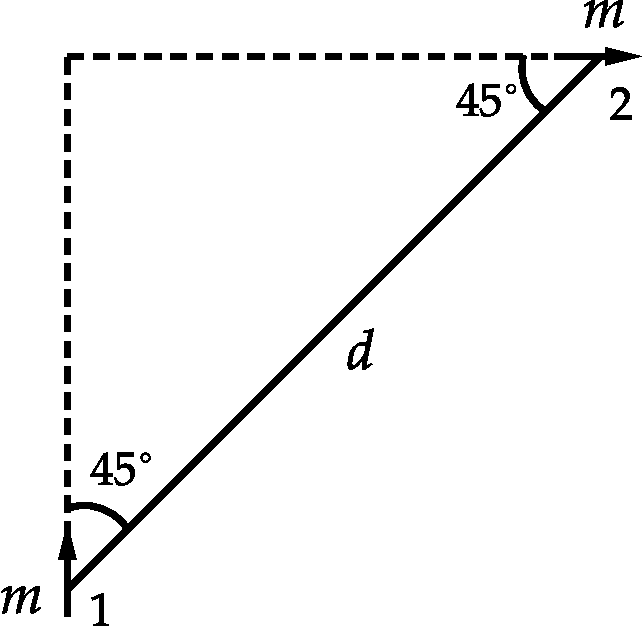
\includegraphics[height=3.5cm,width=4cm]{diagram-20210817(13)-crop}
		\caption{}
		\label{}
	\end{figure}
\end{minipage}
\begin{tasks}(4)
	\task[\textbf{A.}] Zero
	\task[\textbf{B.}]$\frac{\mu_{0} m^{2}}{4 \pi d^{3}}$
	\task[\textbf{C.}]$\frac{3 \mu_{0} m^{2}}{2 \pi d^{3}}$
	\task[\textbf{D.}]$-\frac{3 \mu_{0} m^{2}}{8 \pi d^{3}}$
\end{tasks}
\begin{minipage}{\textwidth}
	\item If a force $\vec{F}$ is derivable from a potential function $V(r)$, where $r$ is the distance from the origin of the coordinate system, it follows that
	\exyear{GATE 2011}
\end{minipage}
\begin{tasks}(2)
	\task[\textbf{A.}]$\vec{\nabla} \times \vec{F}=0$
	\task[\textbf{B.}]$\vec{\nabla} \cdot \vec{F}=0$
	\task[\textbf{C.}]$\vec{\nabla} V=0$
	\task[\textbf{D.}]$\nabla^{2} V=0$
\end{tasks}
\begin{minipage}{\textwidth}
	\item A uniform surface current is flowing in the positive $y$-direction over an infinite sheet lying in $x-y$ plane. The direction of the magnetic field is
	\exyear{GATE 2011}
\end{minipage}
\begin{tasks}(1)
	\task[\textbf{A.}]Along $\hat{i}$ for $z>0$ and along $-\hat{i}$ for $z<0$
	\task[\textbf{B.}]Along $\hat{k}$ for $z>0$ and along $-\hat{k}$ for $z<0$
	\task[\textbf{C.}]Along $-\hat{i}$ for $z>0$ and along $\hat{i}$ for $z<0$
	\task[\textbf{D.}]Along $-\hat{k}$ for $z>0$ and along $\hat{k}$ for $z<0$
\end{tasks}
\begin{minipage}{\textwidth}
	\item A magnetic dipole of dipole moment $\vec{m}$ is placed in a non-uniform magnetic field $\vec{B} .$ If the position vector of the dipole is $\vec{r}$, the torque acting on the dipole about the origin is
	\exyear{GATE 2011}
\end{minipage}
\begin{tasks}(2)
	\task[\textbf{A.}] $\vec{r} \times(\vec{m} \times \vec{B})$
	\task[\textbf{B.}]$\vec{r} \times \vec{\nabla}(\vec{m} \cdot \vec{B})$
	\task[\textbf{C.}]$\vec{m} \times \vec{B}$
	\task[\textbf{D.}]$\vec{m} \times \vec{B}+\vec{r} \times \nabla(\vec{m} \cdot \vec{B})$
\end{tasks}
\begin{minipage}{\textwidth}
	\item Which of the following expressions for a vector potential $\vec{A} \underline{\text { DOES NOT }}$ represent a uniform magnetic field of magnitude $B_{0}$ along the $z$-direction?
	\exyear{GATE 2011}
\end{minipage}
\begin{tasks}(2)
	\task[\textbf{A.}] $\vec{A}=\left(0, B_{0} x, 0\right)$
	\task[\textbf{B.}]$\vec{A}=\left(-B_{0} y, 0,0\right)$
	\task[\textbf{C.}]$\vec{A}=\left(\frac{B_{0} x}{2}, \frac{B_{0} y}{2}, 0\right)$
	\task[\textbf{D.}] $\vec{A}=\left(-\frac{B_{0} y}{2}, \frac{B_{0} x}{2}, 0\right)$
\end{tasks}
\begin{minipage}{\textwidth}
	\item In a constant magnetic field of $0.6$ Tesla along the $\mathrm{z}$ direction, find the value of the path integral $\oint \vec{A} \cdot \overrightarrow{d l}$ in the units of (Tesla $m^{2}$ ) on a square loop of side length $(1 / \sqrt{2})$ meters. The normal to the loop makes an angle of $60^{\circ}$ to the z-axis, as shown in the figure.\\
	\begin{figure}[H]
		\centering
		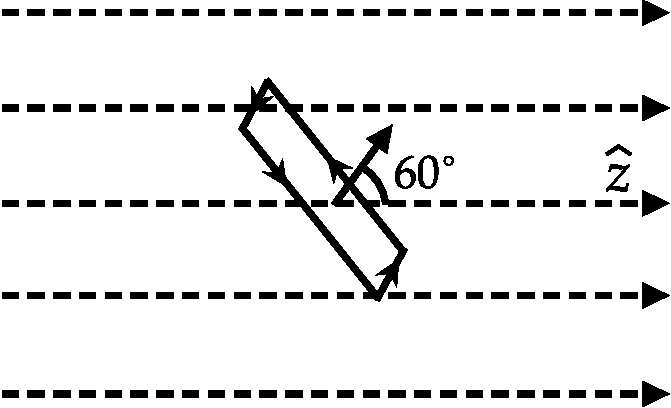
\includegraphics[height=3cm,width=5cm]{diagram-20210817(19)-crop-crop}
	\end{figure}	
	The answer should be up to two decimal places.
	\exyear{GATE}	
\end{minipage}
\begin{minipage}{\textwidth}
	\item The value of the magnetic field required to maintain non-relativistic protons of energy $1 \mathrm{MeV}$ in a circular orbit of radius $100 \mathrm{~mm}$ is Tesla
	\exyear{GATE 2014}
\end{minipage}
\begin{minipage}{\textwidth}
	\item Given that the magnetic flux through the closed loop $P Q R S P$ is $\phi$. If $\int_{P}^{R} \vec{A} \cdot \vec{d} l=\phi_{1}$ along $P Q R$, the value of $\int^{R} \vec{A} \cdot \vec{d} l$ along $P S R$ is
	\exyear{GATE 2015}
	\begin{figure}[H]
		\centering
		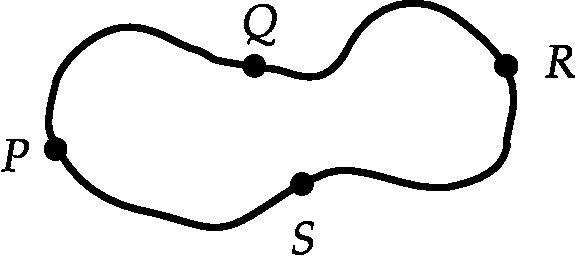
\includegraphics[height=2cm,width=4cm]{diagram-20210818(2)-crop}
	\end{figure}
\end{minipage}
\begin{tasks}(4)
	\task[\textbf{A.}] $\phi-\phi_{1}$
	\task[\textbf{B.}] $\phi_{1}-\phi$
	\task[\textbf{C.}]$-\phi_{1}$
	\task[\textbf{D.}] $\phi_{1}$
\end{tasks}
\begin{minipage}{\textwidth}
	\item Which of the following magnetic vector potentials gives rise to a uniform magnetic field $B_{0} \hat{k} ?$
	\exyear{GATE 2016}
\end{minipage}
\begin{tasks}(4)
	\task[\textbf{A.}] $B_{0} z \hat{k}$
	\task[\textbf{B.}]$-B_{0} x \hat{j}$
	\task[\textbf{C.}]$\frac{B_{0}}{2}(-y \hat{i}+x \hat{j})$
	\task[\textbf{D.}]$\frac{B_{0}}{2}(y \hat{i}+x \hat{j})$
\end{tasks}
\begin{minipage}{\textwidth}
	\item The magnitude of the magnetic dipole moment associated with a square shaped loop carrying a steady current $I$ is $m$. If this loop is changed to a circular shape with the same current $I$ passing through it, the magnetic dipole moment becomes $\frac{p m}{\pi} .$ The value of $p$ is
	\exyear{GATE 2016}
\end{minipage}
\begin{minipage}{\textwidth}
	\item An infinite solenoid carries a time varying current $I(t)=A t^{2}$, with $A \neq 0 .$ The axis of the solenoid is along the $\hat{z}$ direction. $\hat{r}$ and $\hat{\theta}$ are the usual radial and polar directions in cylindrical polar coordinates. $\vec{B}=B_{r} \hat{r}+B_{\theta} \hat{\theta}+B_{z} \hat{z}$ is the magnetic field at a point outside the solenoid. Which one of the following statements is true?
	\exyear{GATE 2017}
\end{minipage}
\begin{tasks}(2)
	\task[\textbf{A.}] $B_{r}=0, B_{\theta}=0, B_{z}=0$
	\task[\textbf{B.}]$B_{r} \neq 0, B_{\theta} \neq 0, B_{z}=0$
	\task[\textbf{C.}] $B_{r} \neq 0, B_{\theta} \neq 0, B_{z} \neq 0$
	\task[\textbf{D.}] $B_{r}=0, B_{\theta}=0, B_{z} \neq 0$
\end{tasks}
\begin{minipage}{\textwidth}
	\item An infinitely long straight wire is carrying a steady current $I$. The ratio of magnetic energy density at distance $r_{1}$ to that at $r_{2}\left(=2 r_{1}\right)$ from the wire is
	\exyear{GATE 2018}
\end{minipage}
\begin{minipage}{\textwidth}
	\item A constant and uniform magnetic field $\vec{B}=B_{0} \hat{k}$ pervades all space. Which one of the following is the correct choice for the vector potential in Coulomb gauge?
	\exyear{GATE 2018}
\end{minipage}
\begin{tasks}(4)
	\task[\textbf{A.}] $-B_{0}(x+y) \hat{i}$
	\task[\textbf{B.}]$B_{0}(x+y) \hat{j}$
	\task[\textbf{C.}] $B_{0} x \hat{j}$
	\task[\textbf{D.}]$-\frac{1}{2} B_{0}(x \hat{i}-y \hat{j})$
\end{tasks}
\begin{minipage}{\textwidth}
	\item  A solid cylinder of radius $R$ has total charge $Q$ distributed uniformly over its volume. It is rotating about its axis with angular speed $\omega$. The magnitude of the total magnetic moment of the cylinder is
	\exyear{GATE 2019}
\end{minipage}
\begin{tasks}(4)
	\task[\textbf{A.}] $Q R^{2} \omega$
	\task[\textbf{B.}]$\frac{1}{2} Q R^{2} \omega$
	\task[\textbf{C.}]$\frac{1}{4} Q R^{2} \omega$
	\task[\textbf{D.}]$\frac{1}{8} Q R^{2} \omega$
\end{tasks}
\begin{minipage}{\textwidth}
	\item An infinitely long wire parallel to the $x$-axis is kept at $z=d$ and carries a current $I$ in the positive $x$ direction above a superconductor filling the region $z \leq 0$ (see figure). The magnetic field $\vec{B}$ inside the superconductor is zero so that the field just outside the superconductor is parallel to its surface. The magnetic field due to this configuration at a point $(x, y, z>0)$ is
	\exyear{GATE 2019}
	\begin{figure}[H]
		\centering
		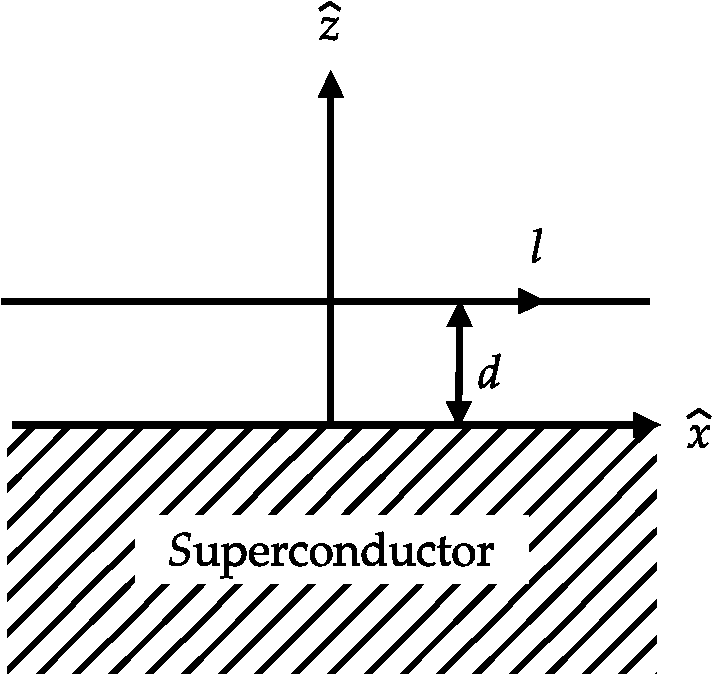
\includegraphics[height=5cm,width=5cm]{diagram-20210818(14)-crop-crop}
		\caption{}
		\label{}
	\end{figure}
\end{minipage}
\begin{tasks}(2)
	\task[\textbf{A.}]$\left(\frac{\mu_{0} I}{2 \pi}\right) \frac{-(z-d) \hat{j}+y \hat{k}}{\left[y^{2}+(z-d)^{2}\right]}$
	\task[\textbf{B.}]$\left(\frac{\mu_{0} I}{2 \pi}\right)\left[\frac{-(z-d) \hat{j}+y \hat{k}}{y^{2}+(z-d)^{2}}+\frac{(z+d) \hat{j}-y \hat{k}}{y^{2}+(z+d)^{2}}\right]$
	\task[\textbf{C.}]$\text { (c) }\left(\frac{\mu_{0} I}{2 \pi}\right)\left[\frac{-(z-d) \hat{j}+y \hat{k}}{y^{2}+(z-d)^{2}}-\frac{(z+d) \hat{j}-y \hat{k}}{y^{2}+(z+d)^{2}}\right]$
	\task[\textbf{D.}]$\text { (d) }\left(\frac{\mu_{0} I}{2 \pi}\right)\left[\frac{y \hat{j}+(z-d) \hat{k}}{y^{2}+(z-d)^{2}}+\frac{y \hat{j}-(z+d) \hat{k}}{y^{2}+(z+d)^{2}}\right]$
\end{tasks}
\begin{minipage}{\textwidth}
	\item The vector potential inside a long solenoid with $n$ turns per unit length and carrying current $I$, written in cylindrical coordinates is $\vec{A}(s, \phi, z)=\frac{\mu_{0} n I}{2} s \hat{\phi}$. If the term $\frac{\mu_{0} n I}{2} s(\alpha \cos \phi \hat{\phi}+\beta \sin \phi \hat{s})$, where $\alpha \neq 0, \beta \neq 0$ is added to $\vec{A}(S, \phi, z)$, the magnetic field remains the same if
	\exyear{GATE 2019}
\end{minipage}
\begin{tasks}(4)
	\task[\textbf{A.}]$\alpha=\beta$
	\task[\textbf{B.}]$\alpha=-\beta$
	\task[\textbf{C.}]$\alpha=2 \beta$
	\task[\textbf{D.}]$\alpha=\frac{\beta}{2}$
\end{tasks}
\begin{minipage}{\textwidth}
	\item A magnetic field $\vec{B}=B_{0}(\hat{i}+2 \hat{j}-4 \hat{k})$ exists at point. If a test charge moving with a velocity, $\vec{v}=v_{0}(3 \hat{i}-\hat{j}+2 \hat{k})$ experiences no force at a certain point, the electric field at that point in SI units is
	\exyear{JEST 2012}
\end{minipage}
\begin{tasks}(2)
	\task[\textbf{A.}] $\vec{E}=-v_{0} B_{0}(3 \hat{i}-2 \hat{j}-4 \hat{k})$
	\task[\textbf{B.}]$\vec{E}=-v_{0} B_{0}(\hat{i}+\hat{j}+7 \hat{k})$
	\task[\textbf{C.}]$\vec{E}=v_{0} B_{0}(14 \hat{j}+7 \hat{k})$
	\task[\textbf{D.}]$\vec{E}=-v_{0} B_{0}(14 \hat{j}+7 \hat{k})$
\end{tasks}
\begin{minipage}{\textwidth}
	\item A small magnet is dropped down a long vertical copper tube in a uniform gravitational field. After a long time, the magnet
	\exyear{JEST 2012}
\end{minipage}
\begin{tasks}(2)
	\task[\textbf{A.}] Attains a constant velocity
	\task[\textbf{B.}] Moves with a constant acceleration
	\task[\textbf{C.}] Moves with a constant deceleration
	\task[\textbf{D.}] Executes simple harmonic motion
\end{tasks}
\begin{minipage}{\textwidth}
	\item A thin uniform ring carrying charge $Q$ and mass $M$ rotates about its axis. What is the gyromagnetic ratio (defined as ratio of magnetic dipole moment to the angular momentum) of this ring?
	\exyear{JEST 2013}
\end{minipage}
\begin{tasks}(4)
	\task[\textbf{A.}] $\frac{Q}{2 \pi M}$
	\task[\textbf{B.}]$\frac{Q}{M}$
	\task[\textbf{C.}]$\frac{Q}{2 M}$
	\task[\textbf{D.}]$\frac{Q}{\pi M}$
\end{tasks}
\begin{minipage}{\textwidth}
	\item The electric and magnetic field caused by an accelerated charged particle are found to scale as $E \propto r^{-n}$ and $B \propto r^{-m}$ at large distances. What are the value of $n$ and $m$ ?
	\exyear{JEST 2013}
\end{minipage}
\begin{tasks}(2)
	\task[\textbf{A.}] $n=1, m=2$
	\task[\textbf{B.}] $n=2, m=1$
	\task[\textbf{C.}]$n=1, m=1$
	\task[\textbf{D.}]$n=2, m=2$
\end{tasks}
\begin{minipage}{\textwidth}
	\item A system of two circular co-axial coils carrying equal currents $I$ along same direction having equal radius $R$ and separated by a distance $R$ (as shown in the figure below). The magnitude of magnetic field at the midpoint $P$ is given by
	\exyear{JEST 2014}
	\begin{figure}[H]
		\centering
		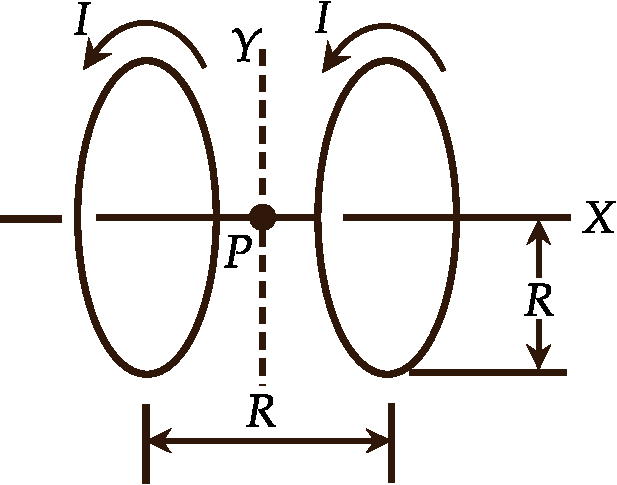
\includegraphics[height=3cm,width=5cm]{diagram-20210809(7)-crop}
		\caption{}
		\label{}
	\end{figure}
\end{minipage}
\begin{tasks}(4)
	\task[\textbf{A.}] $\frac{\mu_{0} I}{2 \sqrt{2} R}$
	\task[\textbf{B.}]$\frac{4 \mu_{0} I}{5 \sqrt{5} R}$
	\task[\textbf{C.}]$\frac{8 \mu_{0} I}{5 \sqrt{5} R}$
	\task[\textbf{D.}] 0
\end{tasks}
\begin{minipage}{\textwidth}
	\item A charged particle is released at time $t=0$, from the origin in the presence of uniform static electric and magnetic fields given by $E=E_{0} \hat{y}$ and $B=B_{0} \hat{z}$ respectively. Which of the following statements is true for $t>0$ ?
	\exyear{JEST 2015}
\end{minipage}
\begin{tasks}(2)
	\task[\textbf{A.}] The particle moves along the $x$-axis.
	\task[\textbf{B.}]The particle moves in a circular orbit.
	\task[\textbf{C.}]The particle moves in the $(x, y)$ plane.
	\task[\textbf{D.}] Particle moves in the $(y, z)$ plane
\end{tasks}
\begin{minipage}{\textwidth}
	\item The strength of magnetic field at the center of a regular hexagon with sides of length $a$ carrying a steady current $I$ is:
	\exyear{JEST 2016}
\end{minipage}
\begin{tasks}(4)
	\task[\textbf{A.}] $\frac{\mu_{0} I}{\sqrt{3} \pi a}$ 
	\task[\textbf{B.}]$\frac{\sqrt{6} \mu_{0} I}{\pi a}$
	\task[\textbf{C.}]$\frac{3 \mu_{0} I}{\pi a}$
	\task[\textbf{D.}]$\frac{\sqrt{3} \mu_{0} I}{\pi a}$
\end{tasks}
\begin{minipage}{\textwidth}
	\item A wire with uniform line charge density $\lambda$ per unit length carries a current $I$ as shown in the figure. Take the permittivity and permeability of the medium to be $\varepsilon_{0}=\mu_{0}=1 . \mathrm{A}$ particle of charge $q$ is at a distance $r$ and is travelling along a trajectory parallel to the wire. What is the speed of the charge?
	\exyear{JEST 2019}
	\begin{figure}[H]
		\centering
		\includegraphics[height=3cm,width=5cm]{jest-crop}
	\end{figure}
\end{minipage}
\begin{tasks}(4)
	\task[\textbf{A.}] $\frac{\lambda}{I}$ 
	\task[\textbf{B.}]$\frac{\lambda}{2 I}$
	\task[\textbf{C.}]$\frac{\lambda}{3 I}$
	\task[\textbf{D.}]$\frac{4 \lambda}{I}$
\end{tasks}
\end{enumerate}

\colorlet{ocre1}{ocre!70!}
\colorlet{ocrel}{ocre!30!}
\setlength\arrayrulewidth{1pt}
\begin{table}[H]
	\centering
	\arrayrulecolor{ocre}
	
	\begin{tabular}{|p{1.5cm}|p{1.5cm}||p{1.5cm}|p{1.5cm}|}
		\hline
		\multicolumn{4}{|c|}{\textbf{Answer key}}\\\hline\hline
		\rowcolor{ocrel}Q.No.&Answer&Q.No.&Answer\\\hline
		1&\textbf{d}&2&\textbf{a}\\\hline
		3&\textbf{a}&4&\textbf{c}\\\hline
		5&\textbf{c}&6&\textbf{0.15}\\\hline
		7&\textbf{1.44}&8&\textbf{b}\\\hline
		9&\textbf{c}&10&\textbf{4}\\\hline
		11&\textbf{d}&12&\textbf{4}\\\hline
		13&\textbf{c}&14&\textbf{c}\\\hline
		15&\textbf{b}&16&\textbf{d}\\\hline
		17&\textbf{d}&18&\textbf{a}\\\hline
		19&\textbf{c}&20&\textbf{c}\\\hline
		21&\textbf{c}&22&\textbf{c}\\\hline
		23&\textbf{d}&24&\textbf{a}\\\hline
	\end{tabular}
\end{table}


























































\newpage
\begin{abox}
	Practise Set-3
\end{abox}
\begin{enumerate}[ label=\color{ocre}\textbf{\arabic*.}]
	\item Consider a coil of radius $R$ is placed in $XY$ plane having current $I$ passing through it. Auppose another coil having the same radius $R$ is placed at a distance $2R$ from the first. Find the magnetic field at the mid point between them?
	\begin{figure}[H]
		\begin{center}
			\includegraphics[width=4cm,height=2cm]{diagram-20210430-crop}
		\end{center}
	\end{figure}
	\begin{answer}
		\begin{align*}
		B \text{at}\quad\text{is}&=B_1+B_2\\
		B_1&=\frac{\mu_{0} I}{2}\times\frac{R^2}{(R^2+R^2)^\frac{3}{2}}\qquad \text{here,}\ z=R\\
		&=\frac{\mu_0 I}{2}\frac{R^2}{2^\frac{3}{2}\times R^3}=\frac{\mu_0 I}{2\times2^\frac{3}{2}\times R}\\
		B_2 \text{ is also }&\text{same}\\
		\therefore B&=2\times\frac{\mu_0 I}{2\times2^\frac{2}{3}R}=\frac{\mu_0I}{2\sqrt{2}R}
		\end{align*}
	\end{answer}
	\item  A very long solenoid with $n$ turns per unit length carries a current $I$. The magnetic field at a point which is on its axis and its end face?
	\begin{figure}[H]
		\begin{center}
			\includegraphics[width=6cm,height=2cm]{diagram-20210430(2)-crop}
		\end{center}
	\end{figure}
	\begin{answer}
		\begin{align*}
		\text{For a  }&\text{solenoid magnetic field  at any point $P$ on its axis is given by}\\
		B&=\frac{\mu_0 nI}{2}(\cos\theta_2-\cos\theta_1)
		\text{$\theta_1$ and $\theta_2$ are the angle made by the end points of the solenoid to $P$.}\\
		\therefore\text{In the  }&\text{case of infinite solenoid,at center}\\
		\theta_1&=\pi,\theta_2=0\\
		\therefore B&=\frac{\mu_0 nI}{2}\times2=\mu_0 nI \quad\text{at center}\\
		\text{Here in }&\text{ this question,at one end}\\
		\theta_1&=\frac{\pi}{2},\quad\theta_2=0 \text{(for long solenoid)}\\
		B&=\frac{\mu_0 n I}{2}\times1=\frac{\mu_0 n I}{2}
		\end{align*}
	\end{answer}
	\item A steady current $I$ flows down a long cylindrical wire of radius $a$ Find the magnetic field, both inside and outside the wire, if\\
	\textbf{(a)} The current is uniformly distributed over the outside surface of the wire.\\
	\textbf{(b)} The current is distributed in such a way that $J$ is proportional to $s$, the distance from the axis.
	\begin{figure}[H]
		\begin{center}
			\includegraphics[width=3.5cm,height=1.5cm]{diagram-20210430(8)-crop}
		\end{center}
	\end{figure}
	\begin{answer}
		\textbf{(a)} Here current is uniform
		\begin{align*}
		\text{Inside the wire \quad $B$}&=\text{$0$\quad $s<a$, no current enclosed} \\
		\text{outside the wire $\oint B\cdot dl$}&\text{$=\mu_0I$}\\
		dl&=2\pi s\\
		\text{s is the radius of }&\text{Amperial loop $dl$ around the wire}\\
		\therefore B\times2\pi s&=\mu_0I\\
		B&=\frac{\mu_0I}{2\pi s}s>a\\
		\end{align*}
		\begin{align*}
		\textbf{(b)}\quad\text{inside the wire}J&=ks\\
		\text{First  we have to find }&\text{  $k$,so}\hspace{3cm}I=\text{total current}\\
		\text{We know}I&=\int_{0}^{a}J\cdot da \hspace{2cm}J=ks \quad da=2\pi s ds\\
		\therefore I&=k2\pi\int_{0}^{a}s^2ds\\
		I&=k2\pi s\frac{s^3}{3}\quad\text{so}\quad k=\frac{3I}{2\pi a^3}\\
		\text{Now inside the wire Consider }&\text{an Amperial loop of radius \ $s$\ inside the wire}\\
		\text{So}\oint B\cdot dl&=\mu_0I \hspace{3cm}J=ks\\
		B\times2\pi s&=\mu_0I\hspace{3cm}ds=2\pi sds\\
		I=\int_{0}^{s}J.ds&=\int_{0}^{s}ks\times2\pi sds\\
		&=k\int_{0}^{s}s^2 ds\times2\pi\\
		&=\frac{ks^3}{3}\times2\pi\\
		\text{Substituting  value }&\text{ of }k\\
		I&=\frac{3 I}{2\pi a^3}\times\frac{s^3}{3}\times2\pi\\
		&=\frac{Is^3}{a^3}\\
		\therefore B\times2\pi s&=\frac{\mu_0Is^3}{a^3}\\
		B&=\frac{\mu_0Is^2}{2\pi a^3}\hat{\phi} \quad \text{inside}\\
		\text{Out side the }&\text{wire}\\
		\oint B\cdot dl&=\mu_0I\\
		B\times2\pi s&=\mu_0I\\
		B&=\frac{\mu_0I}{2\pi s}\hat{\phi}
		\end{align*}
	\end{answer}
	\item Find the magnetic field at the center $O$ for the following figures.\\
	\begin{minipage}{0.45\textwidth}
		\begin{figure}[H]
			\begin{center}
				\includegraphics[width=3.5cm,height=3.5cm]{diagram-20210430(1)-crop}
			\end{center}
			\caption{(a)}
		\end{figure}
	\end{minipage}
	\begin{minipage}{0.45\textwidth}
		\begin{figure}[H]
			\begin{center}
				\includegraphics[width=3.5cm,height=3.5cm]{diagram-20210430(4)-crop}
			\end{center}
			\caption{(b)}
		\end{figure}
	\end{minipage}
	\begin{answer}
		\begin{align*}
		\textbf{(a)}\quad\text{Field at $O$ due to }&\text{$PS$ and $QR$ is zero. Because the point $O$ lies along the axis of the segment.}\\
		\text{Field at $O$ due }&\text{to $RS$,}\\
		B_1&=\frac{\mu_0I}{2b}\times\frac{\phi}{2\pi}\\
		\text{Field at $O$ due }&\text{to $PQ$}\\
		B_2&=\frac{\mu_0I}{2a}\times\frac{2\pi-\phi}{2\pi}\\
		\text{So total field }&\text{at B}\\
		B&=B_1+B_2\\
		&=\frac{\mu_0I}{4\pi}\left( \frac{\phi}{b}+\frac{2\pi-\phi}{a}\right) \\
		\end{align*}
		\begin{align*}
		\textbf{(b)}\quad\text{Field at $O$ due to }&\text{arc $pQ$}\hspace{2cm}\\
		B_1&=\frac{\mu_0I}{2a}\times\frac{3\frac{\pi}{2}}{2\pi}\\
		=&\frac{\mu_0I}{2a}\times\frac{3}{4}\\
		\text{Field at $O$ due to $PT$ and } &\text{$QR$ are zero. Field at $O$ due to $ST$ and $RS$.}\\
		B_2=\ B_3&=\frac{\mu_0I}{4\pi b}(\sin\theta_2-\sin\theta_1)\\
		&=\frac{\mu_0I}{4\pi b}\sin45\hspace{3cm}\theta_2=45,\quad \theta_{1}=0\\
		&=\frac{\mu_0I}{4\pi b}\times\frac{1}{\sqrt{2}}\\
		\text{Total field at \ $O$,}\\
		B&=B_1+B_2+B_3\\
		&=\frac{\mu_0I}{2a}\times\frac{3}{4}+2\times\frac{\mu_0}{4\pi b}\times\frac{1}{\sqrt{2}}\\
		&=\frac{\mu_0I}{4\pi}\left[\frac{3\pi}{2a}+\frac{\sqrt{2}}{b} \right] 
		\end{align*}
	\end{answer}
	\item Magnetic field at center $O$ due to a regular pentagon if $I$ current flowing through it and $R$ be the distance from each side to $O$.
	\begin{figure}[H]
		\begin{center}
			\includegraphics[width=2.5cm,height=2.5cm]{diagram-20210430(5)-crop}
		\end{center}
	\end{figure}
	\begin{answer}
		For an $n$ sided rectangular polygon field at center\\
		$B=\frac{n\mu_0I}{2\pi R}\tan\frac{\pi}{n}$ if $R$ become the distance from each vertex to center\\
		if $R$ is the distance from each side to center  
		\begin{align*}
		B&=\frac{n\mu_0I}{2\pi R}\sin\frac{\pi}{n}\\
		\text{Here,}\quad n&=5\quad \\
		\text{Then,} B&=\frac{\mu_0nI}{2\pi R}\sin\frac{\pi}{n}\\
		&=\frac{5\mu_0 I}{2\pi R}\sin\frac{\pi}{5}\\
		&=\frac{5\mu_0I}{2\pi R}\sin 36	
		\end{align*}
	\end{answer}
	\item Thick slab extending from $z=-a$ and $z=+a$ carries a uniform volume current $J=J(x) $.Find the magnetic field as a function of $Z$ both inside and outside the slab.
	\begin{figure}[H]
		\begin{center}
			\includegraphics[width=5cm,height=3cm]{diagram-20210430(6)-crop}
		\end{center}
	\end{figure}
	\begin{answer}
		Consider an Amperian loop of length $l$ and height $z$, applying Ampere's law.\\
		\begin{align*}
		\oint B\cdot dl&=\mu_0I\\
		B\times l&=\mu_0\cdot lz\cdot J\hspace{3cm}I=lz\cdot \vec{J}\\
		\therefore B&=\mu_0Jz\hat{y}\hspace{3cm}(-a<z<a)
	\intertext{	By using right hand thumb rule we can say that for $z>0$ field is along $-y$ direction and for $z<0$ field is along $+y$ direction}
		\text{So}\quad B&=-\mu_0Ja\hat{y}\quad\text{for}\quad z>+a\\
		B&=+\mu_0Ja\hat{y}\quad\text{for}\quad z>-a
		\end{align*}
		By consideting an Amperian loop of length $l$ and height $a$.
	\end{answer}
	\item A beam of proton with velocity $4\times10^5 {m}/{Sec}$enters a uniform magnetic field of 0.3Tesla at an angle $60^\circ$to the magnetic field. Find the radius of the helical path taken by the proton beam. Also find the pitch of the helix.\\
	\begin{answer}
		\begin{align*}
		V=4\times10^5 \frac{m}{Sec}\hspace{1cm}V_\perp&=V\sin60\hspace{1cm}V_\parallel=V\cos60\\
		\frac{mv_\perp^2}{R}&=qv_\perp B\\
		R&=\frac{m v_\perp}{qB}\\
		&=0.012m \quad m_p=1.6\times 10^{-27}kg\\
		\text{Pitch of}&\text{ helix,}\\
		d&=V_\parallel T=V_\parallel\times\frac{2\pi m}{qB}=0.044m
		\end{align*}
	\end{answer}
	\item The maximum energy of deuteron coming out of a cyclotron accelerator is $20MeV$. The maximum energy of proton that can be obtained from the accelerator is?
	\begin{answer}
		\begin{align*}
		KE_{max}&=\frac{Q^2B^2R^2}{2m}\\
		KE_d&=20 MeV\\
		KE_P&=?\\
		20&=\frac{1\times B^2\times R^2}{2\times2}\\
		KE_P&=\frac{1\times B^2\times R^2}{2\times1}\\
		KE_P&=20MeV
		\end{align*}
	\end{answer}
	\item Ab $\alpha$ particle is accelerated by potencial difference of $10^4V$. Find the change in its direction of motion. If it enters normally in a region of thickness $0.1m$ having transverse magnetic induction of $0.1 $Tesla$(m=6.4\times10^-27kg)$
	\begin{figure}[H]
		\begin{center}
			\includegraphics[width=3cm,height=3cm]{diagram-20210430(9)-crop}
		\end{center}
	\end{figure}
	\begin{answer}
		Before entering the field, $\alpha$ particle is accelerated by a potential difference of $10^4V$ then\begin{align*}
		\frac{1}{2}mu^2&=qV\\
		u&=\sqrt{\frac{2qV}{m}}\\
		R&=\frac{mu}{QB}=\frac{m}{QB}\sqrt{\frac{2qV}{m}}\quad V=pd\\
		&=\frac{1}{B}\sqrt{\frac{2mV}{q}}\\
		\text{$ \theta $ is the angle }&\text{of deflection,}\\
		\therefore\sin\theta&=\frac{l}{R}\hspace{3cm}V=10^4\text{Volt}\\
		\sin\theta&=0.1\times B\times\sqrt{\frac{q}{2mV}}\\
		q&=2\times1.6\times10^{-16}=3.2\times10^{-16}c\\
		m&=6.4\times10^{-27}kg\\
		\sin\theta&=0.1\times0.1\times\sqrt{\frac{3.2\times10^{-16}}{2\times6.4\times10^{-27}\times10^4}}\\
		&=\frac{1}{2}\\
		\therefore\theta&=30^\circ
		\end{align*}
	\end{answer}
	\item There are two similar coils at $P$ and $Q$ having same no of turns located at $(0,4,0)$ and$(0,0,3)$. Area of crone section are in the ratio $4:3$.A $16 A$ current flowing through coil $P$in clockwise direction and a $9\sqrt{3} A$ current in $Q$ in anticlockwise direction . What will the deflection of a compass needle placed at the origin. Assumes that earth field is negligible and radius of the coil are very small compared to their distance from the origin.
	\begin{figure}[H]
		\begin{center}
			\includegraphics[width=5cm,height=4cm]{diagram-20210430(7)-crop}
		\end{center}
	\end{figure}
	\begin{answer}
		\begin{align*}
		\text{$B$ at a distance}&\text{ $x$ from a coil of radius $r$}\\
		B&=\frac{\mu_0I}{2}\frac{nr^2}{(r^2+x^2)^\frac{3}{2}}\\
		&=\frac{\mu_0 \ln \pi r^2}{2\times\pi \times(x^2)^\frac{3}{2}}\hspace{1cm}\quad \text{When}\ r<<<x\\
		&=\frac{\mu_0In\times A}{2\pi x^3}\\
		\text{Field at 'o' \ due }&\text{to $P$,}\\
		B_P&=\frac{\mu_0\times16\times A_P}{2\pi\times4^3}\\
		\text{Field at 'o' \ due }&\text{to $Q$,}\\
		B_Q&=\frac{\mu_0\times9\sqrt{3}\times A_Q}{2\pi\times3^3}\\
		\text{From figure resultant of $B_P$ }&\text{and $B_Q$, $B$ makes an angle With \ $B_Q$\ with \ $B_P$}\\
		\tan\theta&=\frac{B_Q}{B_P}
		=\frac{\mu_0\times9\sqrt{3} A_Q}{2\pi\times3^3}\times\frac{2\pi\times4^3}{\mu_0\times16\times A_P}\\
		\tan\theta&=\sqrt{3}\\
		\theta&=60^\circ
		\end{align*}
	\end{answer}
\end{enumerate}